\documentclass[a4paper, oneside, 11pt]{report}
\usepackage{epsfig,pifont,float,multirow,amsmath,amssymb}
\newcommand{\mc}{\multicolumn{1}{c|}}
\newcommand{\mb}{\mathbf}
\newcommand{\mi}{\mathit}
\newcommand{\oa}{\overrightarrow}
\newcommand{\bs}{\boldsymbol}
\newcommand{\ra}{\rightarrow}
\newcommand{\la}{\leftarrow}

\usepackage{algorithm}
\usepackage{algorithmic}
\usepackage{graphics}
\usepackage{placeins}
\usepackage{float}

\topmargin = 0pt
\voffset = -80pt
\oddsidemargin = 15pt
\textwidth = 425pt
\textheight = 750pt

\begin{document}

\begin{titlepage}
\begin{center}
\rule{12cm}{1mm} \\
\vspace{1cm}
{\large  CMP-7009A Advanced Programming Concepts and Techniques}
\vspace{7.5cm}
\\{\Large Project Report - 12th January, 2023}
\vspace{1.5cm}
\\{\LARGE Interpreter for Maths Visualisation Software - MathChamp}
\vspace{1.0cm}
\\{\Large Group Members: \\ Christopher Gavey, Ebin Paul, Max James, Aswin Sasi, Soniya Avarachan}
\vspace{1.0cm}
\\{\Large https://github.com/paul3bin/maths-interpreter}
\vspace{8.0cm}
\\{\large School of Computing Sciences, University of East Anglia}
\\ \rule{12cm}{0.5mm}
\\ \hspace{8.5cm} {\large Version 1.0}
\end{center}
\end{titlepage}

\setcounter{page}{1}

\tableofcontents


\begin{abstract}
This project aimed to develop an intuitive Python-focused Mathematical Interpreter, \emph{MathChamp}, with an interactive Graphical User Interface (GUI) utilising \emph{PyQt5}. The first step was researching similar interpreters, such as \emph{MATLAB}. Following the analysis of approaches and completing the design process, lexical analysis was planned in detail and developed. Upon completion of the lexer, an abstract syntax tree (AST) was generated for syntactic analysis and integrated. The GUI was designed, developed, and integrated in the next stage with the core \emph{MathChamp} program. The final step of implementation was visualising expressions with settings-rich plots and implementing additional features. Throughout the project, \emph{MathChamp} followed the agile scrum methodology for consistent iterative and incremental development (IID) across the project life cycle. The project was split into development sprints, and roles were allocated for these sprints across the development team, with set and measured goals and deadlines. The final \emph{MathChamp} solution delivers a modern and powerful user interface where users can enter expressions, statements, and commands with function calls using custom syntax. Variables can be defined, manipulated, and visualised, and additional features include zero crossings, factorials, and Boolean operations.
\end{abstract}


\chapter{Introduction} \label{chap:intro}

\section{Project statement}
This project will utilise the \emph{Python} programming language to develop a maths interpreter solution. The interpreter, \emph{MathChamp}, will evaluate expressions, support functionality for defining variables, calling predefined functions, and visualising functions of two or more variables on a plot in the form of \emph{y=f(x)}. Users will be able to enter expressions, statements and commands with function calls using a custom syntax, and make changes to plotting utilising helpful graphic settings. The modern and intuitive graphical user interface (GUI) will be developed using \emph{PyQt5}. 

At a minimum, weekly meetings will be set to discuss the project's progress, issues and bugs, testing, delegated tasks, and, finally, to evenly delegate new tasks (upon completion of those previously assigned). The final deliverable will support additional functionality, as detailed in the MoSCoW below.


\section{MoSCoW}
\textbf{MUST HAVE:} \label{MoSCoW-must}
\begin{itemize}
    \item Well tested, well documented software
    \item Clean code
    \item Intuitive GUI
    \item Variable assignment (and visualisation)
    
    \item Accurate BODMAS Order of Operations/Precedence
    \item Visualisation of Mathematical Functions
\end{itemize}

Firstly, the maths interpreter's core functionality and user experience will be the focus; with any additional features outlined in the 'should' or 'could' sections being addressed in future sprints depending on progress. Following an iterative and incremental Development (IID) cycle, the code will be tested regularly as functionality and features are added over time through unit testing and manual test where necessary (mostly for the GUI). Before implementing additional features, the code will be improved to increase efficiency, check for logic errors in calculations, and to ensure good coding practice is used.\\

\textbf{SHOULD HAVE:} \label{MoSCoW-should}
\begin{itemize}
    \item All basic arithmetic expressions 
    \item Excellent Graphical User Interface (GUI)
    \item Professionally presented plots with configuration settings
\end{itemize}

The interface and visualisation of functions will follow great design principles, plotting will provide multiple intuitive settings including zoom, subplot configuration, editable axis and curve parameters, view reset, and the ability to save the view. \\

\textbf{COULD HAVE:} \label{MoSCoW-could}
\begin{itemize}
    \item Logical/Boolean Expressions
    \item Factorials
    \item Zero Crossings
    \item Polar Curve Spirograph
    \item Operations on Matrices
\end{itemize}
For additional functionality, first Boolean expressions will be prioritised for integration into the interpreter, followed by zero crossings. If within the time-frame of the project delivery date, operations on matrices and a Spirograph in polar coordinates will too be explored. However, additional unconsidered features may also be implemented if they provide useful functionality to the interpreter.\\

\textbf{WONT HAVE:} \label{MoSCoW-wont}
\begin{itemize}
    \item Complex Numbers 
    \item Differentiation
\end{itemize}
Due to group changes, three weeks of combined development time was absent. Therefore, complex numbers and differentiation will not be considered for implementation as additional features because of the considerable overhead, and therefore risk of not meeting the project due date to a high standard.\\


\section{Report structure}
The remainder of this report will be structured as follows: Background information on the MathChamp interpreter will be discussed, followed by lo-fi and medium-fi designs. The methodologies utilised in development will then be introduced and explained in detail, followed by the stages of implementation sprint-by-sprint and how each sprint correlates to the specific methodologies (where necessary). Next, the testing stages of the interpreter will be explored and discussed in detail. Finally, a project conclusion and discussion will be covered, along with individual contributions to the project. Appendices such as UML diagrams and test plans will appear at the end of the report.


\chapter{Background}\label{background}

\section{Background}
Various background resources have been used to understand the theoretical underpinnings of the techniques applied, namely, lexical and syntactic analysis. All resource references can be found in in the Bibliography following Chapter \ref{bibliography}. The references have also been included in the code files they're applicable to; appearing at the top of the program as a comment. Of all resources, the most helpful in the development of MathChamp was the presentation slides from Lecture 2: Programming Languages, especially those covering interpreters and compilers, slides 26 - 82. The knowledge learnt from the slides and lectures was combined with further research on the design and development of lexical and syntactic analysis. The conducted research included blogs on lexing and parsing processes to provide some real-world insight into how the development of MathChamp could be tackled and planned for appropriately. MATLAB was too closely studied to assist in aligning the expectations and goals of an intuitive mathematical interpreter.


\chapter{Methodology}\label{Methodology}

\section{Method 1 - Agile Scrum}
The development of MathChamp was split over four major sprints, between one or two weeks, as discussed in chapter \ref{Implementation}. The Agile Scrum methodology was closely followed. Once the goals of MathChamp were determined as a team and clear sprint goals defined, work began. No specific team member was allocated the role of scrum master. However, each member regularly checked on the progress of other members as relevant to them. For example, the team member responsible for the GUI discussing progress with the members responsible for the core program and vice versa, to aid in integrating the systems and completion in a similar time-frame.

Weekly group meetings were held each Saturday and Wednesday for two hours at noon, and attended consistently by most members. To begin the meetings, progress since the last meeting was first discussed, along with any issues faced in completing the allocated tasks member by member. Issues faced, primarily technical, were often resolved in these meetings, therefore a critical tool in our progress. Once tasks had been completed and new functionality developed, this was tested before and after implementation into the core program by the team member responsible for rigorous testing. Upon completion of all allocated tasks for a sprint, a sprint retrospective was conducted to discuss the following: 

\begin{enumerate}
    \item What went well? 
    \item What can we improve? 
    \item How can we improve it?
\end{enumerate}

The next sprint would then be planned with a set of appropriate goals, a deadline, and evenly distributed tasks amongst the team. Before closing each meeting, the location and time would be confirmed for the next, and an email reminder/calendar item would be sent out to all team members using the Booker System. For general communication, a WhatsApp group was utilised from the beginning to address any questions or issues in between meetings.


\section{Method 2 - GitHub}
GitHub was, arguably, the most critical collaboration tool employed. At the beginning of development, a repository was setup, and each group member was added. In the beginning, three branches were setup; main; development; and testing. The team members also setup GitHub Desktop and connected the repository on each of their computers to further aid collaboration. Once new code was developed, it would first be uploaded to development and then be tested by team member responsible for all the testing. Upon confirmation that the code was functional, reliable, and bug-free, and the test plan updated, it would then be uploaded to the main branch. Following sprint one, branches were created for the GUI, functions, and plotting. Bugs, enhancements, important goals, and documentation were listed in the Issues Module of the repository, regularly kept up to date, and closed once completed. This was especially important in identifying, logging, and tracking bugs, which were easily accessed by utilising GitHub desktop and the Visual Studio Code GitHub Plugin. As the project progressed and dependencies grew, a helpful README file was uploaded with instructions for downloading the MathChamp program, creating a virtual environment (venv), and installing dependencies.


\section{Method 3 - Abstract Syntax Tree (AST)}

\begin{figure}[H]
    \centering
    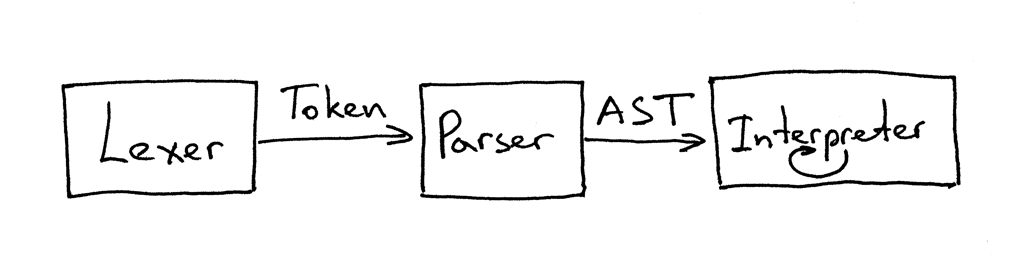
\includegraphics[height=3.5cm]{expressionProcess.png}
    \caption{Expression Processing}
    \textit{ruslanspivak.com}
    \label{fig:expressionprocessing}
\end{figure}

The Abstract Syntax Tree data structure was utilised for the interpreter to generate the machine code from the list of tokens. The tokens are parsed, and the root node of the syntax tree is returned, following the BODMAS order of operations to ensure correct precedence. An input string is collected from the user and calls the Interpreter Class, which is instantiated with the input string. The Lexer first creates a list of characters from the user input string. The input string is looped through to identify each token using the Generate\_Tokens method in the Lexer Class; the Get\_Tokens method then returns the list of tokens. The Interpreter Class gets the list of tokens and creates an object of the Parser Class (which passes the list of tokens). The AST is created from this list and returns the root node of the tree, as shown in figure \ref{fig:AST}.

\begin{figure}[H]
    \centering
    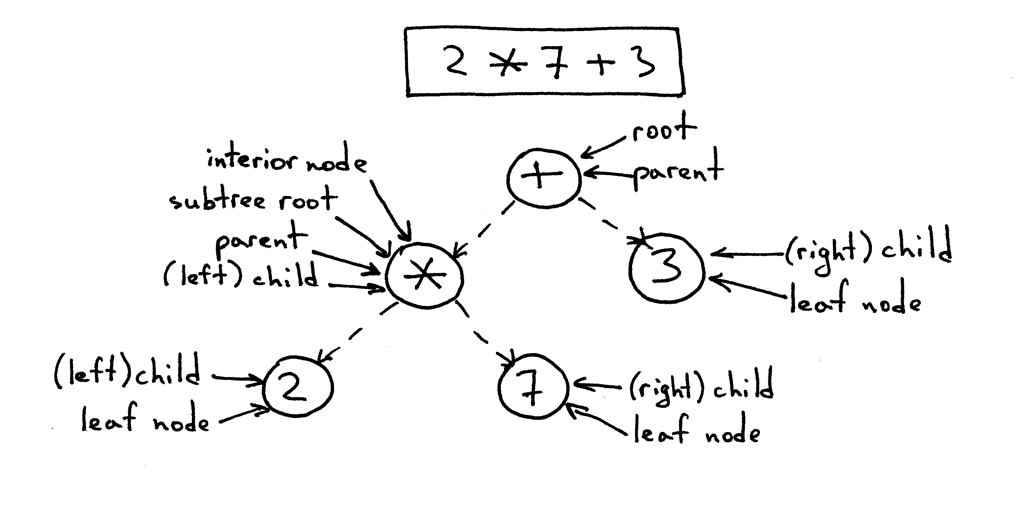
\includegraphics[width=16.0cm]{AST.png}
    \caption{Abstract Syntax Tree}
    \textit{ruslanspivak.com}
    \label{fig:AST}
\end{figure}

\newpage

\subsection{Polymorphism} 
Each class in the Nodes.py file has its own Get\_Node\_Value method and a Magic/Dunder method. This approach was selected so that rather than checking the token type of each node (such as Integer or Float), calling the method Get\_Node\_Value will return the node's value regardless of its class. By using our OperandNode class, this bypasses the requirement to create a different node class for every operator. In turn, this increased the code readability and maintainability, but more importantly, reduced execution time. Get\_Node\_Value is shown below in figure \ref{fig:operandnodeclass}, in the OperandNode class.

\begin{figure}[H]
    \centering
    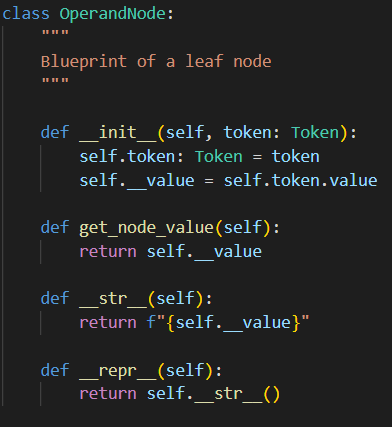
\includegraphics[width=8cm]{MethodOverloading.png}
    \caption{OperandNode Class}
    \label{fig:operandnodeclass}
    \textit{nodes.py}
\end{figure}

\section{Method 4 - PyQt5}
The critical tool employed for the development of the intuitive Graphical User Interface is the \emph{PyQt} \emph{Python} binding (PySide6) of the multi-platform Qt framework. \emph{PyQt5} is by far the most prevalent library to employ in a \emph{Python}-based application requiring a modern GUI that functions well on a large assortment of devices \cite{qt2022}. Whilst the \emph{Tkinter} \emph{Python} binding is easier to use, it lacks much of the advanced functionality available in \emph{PyQt5}. The desired level of advanced user interface design with in-depth tooling and overall functionality was not possible with \emph{Tkinter}. However, besides more complex implementation, a disadvantage of \emph{PyQt5} is that \emph{Tkinter} is built into \emph{Python}, whereas \emph{PyQt5} is not and therefore requires a virtual environment (venv). Nevertheless, the additional time invested in implementing \emph{PyQt5} has paid off in delivering a modern, intuitive, and functionally scalable solution that despite being developed on a \emph{Mac}, has been portable to \emph{Windows} machines. 

\newpage
\subsubsection{Matplotlib}
Whist \emph{PyQtGraph} is a popular choice for plotting functionality in \emph{Python}, it does not deliver even somewhat close to the graphic quality made possible with \emph{Matplotlib}. The main benefit of \emph{PyQtGraph} is the fast execution speed; however, it is more focused on data acquisition and analysis in engineering applications, often for graphs that require constant updating \cite{pyqtgraphdevs2022}. For our mathematical interpreter, \emph{MathChamp}, \emph{Matplotlib} was the better option as it is geared towards \emph{MatLab} programming, focusing on features, settings, and one-off plots. Paired with the advanced functionality of \emph{PyQt5} system support, it was the obvious choice. Our plotting function buttons give users the options to: pan in and out, alter subplot configurations, edit axis and curve parameters, reset their plot view following alterations, style graphs with a variety of line styles and colours, alter titles and labels, and save their custom plot. In addition, they can hover over graph points to display the values of the X and Y in real-time.


\section{Method 5 - RegEx}

\begin{figure}[H]
    \centering
    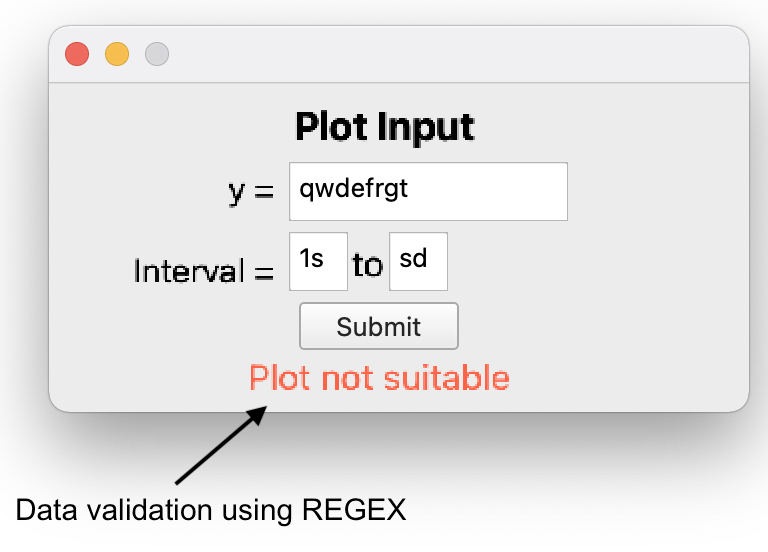
\includegraphics[width=7cm]{regex.png}
    \caption{Showing REGEX being used to data validation}
    \label{fig:regex_validation}
\end{figure}

Regular expressions (RegEx) are employed to perform data validation on the pop-up windows, such as for Variable Assignment and Plotting. Therefore, users who are not familiar with the syntax of our custom language can use still use and interact with \emph{MathChamp} thanks to increased accessibility. The data validation will prevent them from inputting invalid data into fields, such as entering the value of a variable as a String rather than an Integer or Float. In addition, error messages were included in \emph{MathChamp} to guide users when they make input errors for performing the expressions themselves, such as entering an \& or \}.


\section{Method 6 - Zero Crossing}\label{zero-crossing-sec}
It was decided to use the bisection method of finding zero crossings over the Newton-Raphson due to time constraints. This gives us an approximation of the crossing by diving the interval multiple times until a value close enough is reached. Please refer to figure \ref{fig:bisection}, on the following page.

\begin{figure}[H]
    \centering
    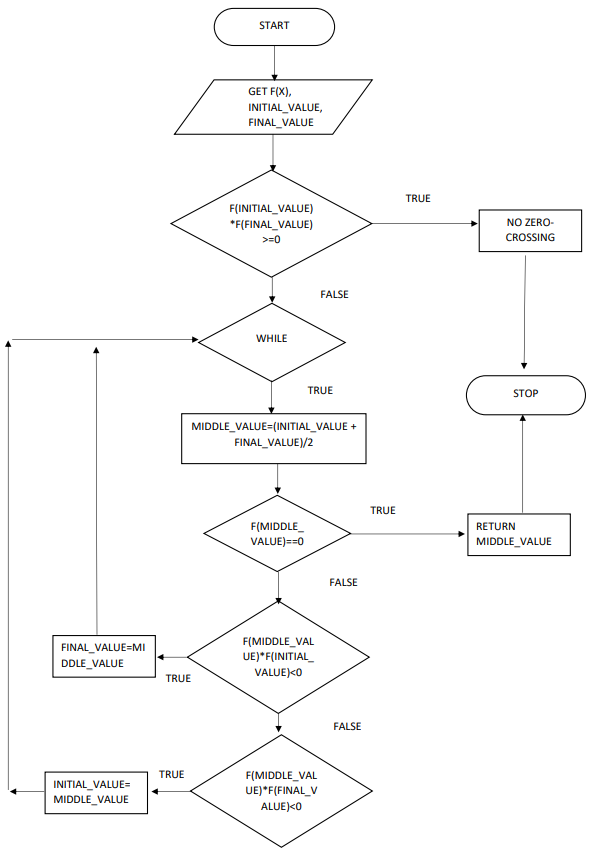
\includegraphics[width=16cm]{BisectionMethod.png}
    \caption{Bisection Method for Zero Crossings}
    \label{fig:bisection}
\end{figure}
\FloatBarrier

\section{Method 7 - Variable dependency}\label{variable-dep-sec}

During development, it was brought to our attention that there was a way variables could be implemented that would mean that they have dependencies on one another. For example, if \emph{'variable2'} is assigned the value of \emph{'variable1'} the value of \emph{'variable2'} should change as well. During the final sprint, one of the group members completed all their allocated tasks so they decided to spend their time implementing this functionality.

\begin{figure}[H]
    \centering
    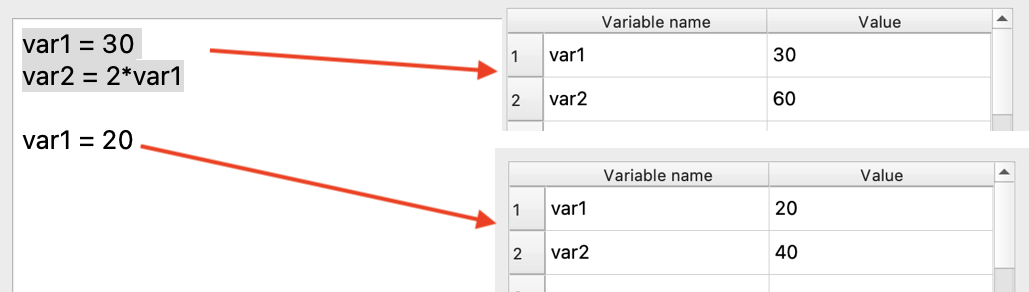
\includegraphics[width=13cm]{variabledep.png}
    \caption{Showing variable dependency in our software}
    \label{fig:variable_dep}
\end{figure}

The way this was achieved was by expanding what information is stored within the program once a variable is declared. Previously, only the variable name and is value were stored within a dictionary; now there's two other dictionaries; one storing the variable name and the statement used to define it, and another with the variable name and a list which holds the names of the variables that have a dependency to the variable within the dictionary key. 

\chapter{Implementation}\label{Implementation}

\section{Early sprints}

For all sprints, a Gantt chart was used to keep track of what tasks were remaining and within what sprint, as shown in Appendix \ref{gantt}. 

\subsection{Sprint 1 (17/10/2022)}
The first sprint of the MathChamp interpreter began at the start of the fourth week of the project timeline, on the 17th of October, 2022, a new group was formed following the withdrawal of our previous members. In turn, it was decided that due to most of the group's familiarity with \emph{Python}, this would be the ideal language to develop in and ensure a robust and feature-rich interpreter solution. 

The initial focus for this sprint is the lexical analyser/tokeniser. Our goal for completion of this sprint is the 24th of October, 2022 (1 week). Only the foundational tokens for MathChamp will be focused on at this stage. Therefore, the following tokens for identification and categorisation will be defined:

\begin{itemize} \label{InitialTokens}
    \item INTEGER = \textit{"INTEGER"}
    \item PLUS = \textit{"PLUS"}
    \item MINUS = \textit{"MINUS"}
    \item MULTIPLY = \textit{"MULTIPLY"}
    \item DIVIDE = \textit{"DIVIDE"}
    \item LEFT\_PARENTHESIS = \textit{"LEFT\_PARENTHESIS"}
    \item RIGHT\_PARENTHESIS = \textit{"RIGHT\_PARENTHESIS"}
    \item FLOAT = \textit{"FLOAT"}
    \item END = \textit{"END"}
\end{itemize}

\begin{figure}[h]
    \centering
    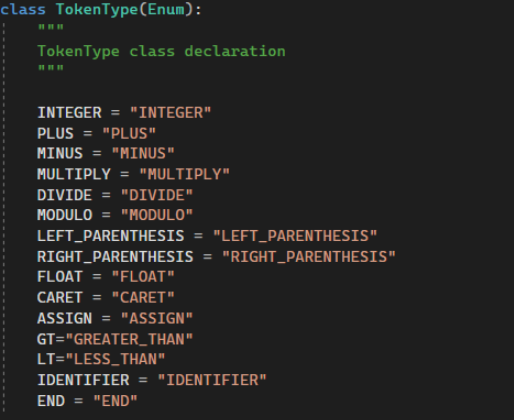
\includegraphics[width=12.0cm]{tokenClass1.png}
    \caption{Completed Lexical Analyser - TokenType (Token.py)}
    \label{fig:bnf}
\end{figure}
\newpage

\begin{figure}[h]
    \centering
    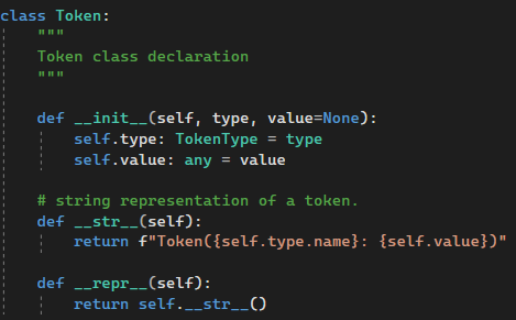
\includegraphics[width=12.0cm]{tokenClass2.png}
    \caption{Lexical Analyser - Token (Token.py)}
    \label{fig:bnf}
\end{figure}

As this project is of a large sizethe group was behind due to external factors such as group members changing modules and degrees, so tasks were divided so while one team member was working on the lexer and parser, another was developing UML class diagrams so that the flow of the system at a high-level could be understood to make development run smoother. This can be evidenced in Appendix \ref{uml-diagrams}.

\subsection{Sprint 2 (24/10/2022)}
Lexical analysis of the above foundational tokens was successful by the deadline. The second sprint begins on the 24th of October, 2022. It will first primarily focus on the expansion of the lexer tokens. Following this, the Abstract Syntax Tree (AST) will be defined from the identified tokens, and the syntactic analysis/parser will be developed. The deadline for completion will be set as the 30th October, 2022.

The following tokens will be added:

\begin{itemize}
    \item CARET = \textit{"CARET"}
    \item IDENTIFIER = \textit{"IDENTIFIER"}
    \item ASSIGN = \textit{"ASSIGN"}
    \item MODULO = \textit{"MODULO"}
\end{itemize}

\begin{figure}[h]
    \centering
    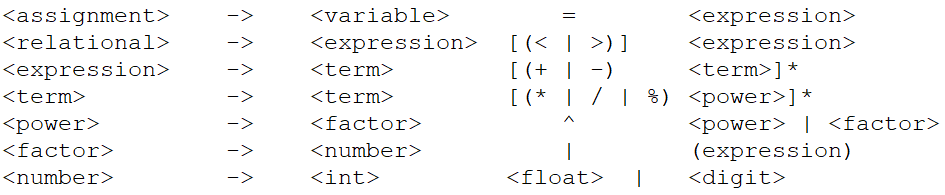
\includegraphics[width=14.5cm]{BNF.png}
    \caption{Syntax Analyser Backus–Naur Form}
    \label{fig:bnf}
\end{figure}

\begin{figure}[h]
    \centering
    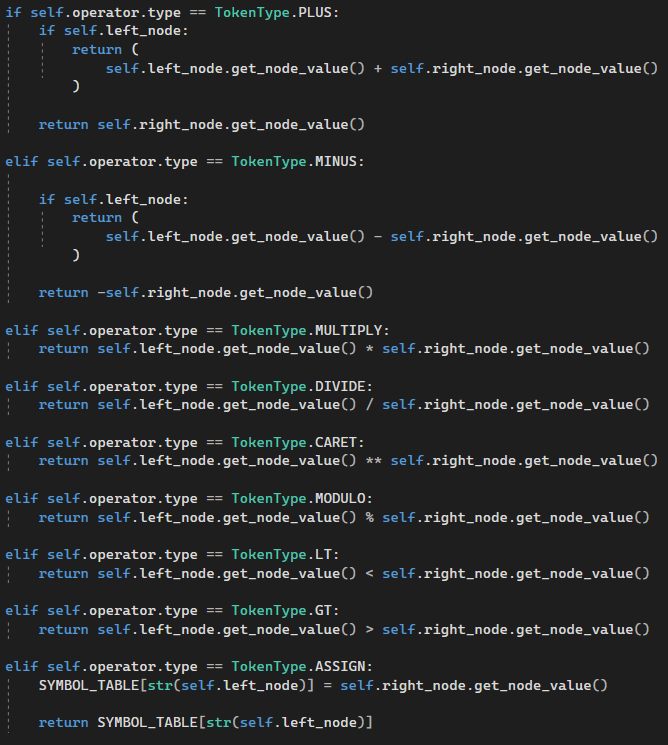
\includegraphics[width=12.0cm]{nodeValue.png}
    \caption{Syntax Analyser - Operator Node Class (Nodes.py)}
    \label{fig:bnf}
\end{figure}

\textbf{31/10/2022}:\\ \\
The deadline for completing the above tasks was met, the remainder of the lexical analyser was completed, and the parser was implemented successfully. The functionality of expressions was thoroughly tested using the manual test plan. A few precedence issues were discovered which caused logic errors, such as the CARET\^\ operator; the issues were actioned and tested again to ensure correct, accurate functionality.

Next sprint task:
As the basic functionality of MathChamp is now in place, developing the Graphical User Interface (GUI) utilising PyQt5 is the next focus. The first Lo-Fi design will be drawn up, and feedback will be collected from the group members to make changes to the design of the main window, variable assignment window, script window, and plotting window. Following this, a Medium-Fi design will be created in Microsoft Visio. Development of the interface will then begin following the agreed design specifications. The deadline for the GUI to be completed will be set as the 6th November, 2022.


\section{Midway sprints}
\subsection{Sprint 3 (07/11/2022)}

\begin{figure}[H]
    \centering
    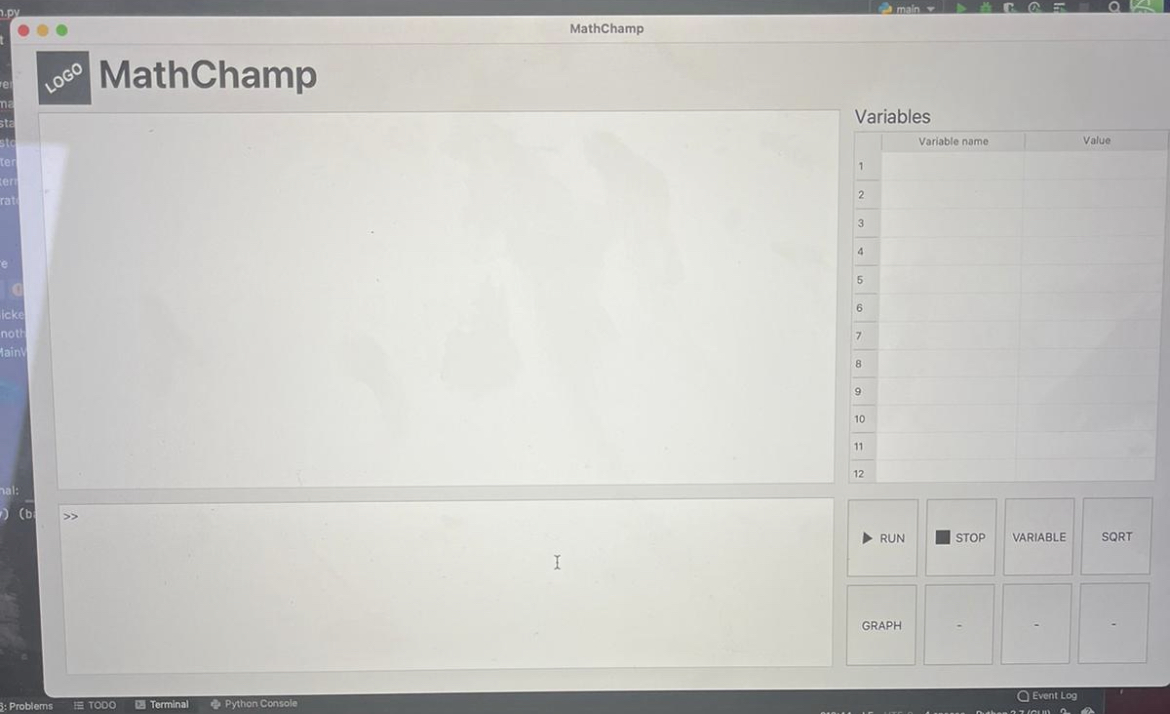
\includegraphics[width=12cm]{1st_screenshot.jpg}
    \caption{1st iteration of GUI from Sprint 3}
    \label{fig:1stGUI}
\end{figure}

MathChamp is now at a stage where it has a working lexer, parser, and GUI (ready to be integrated with the main program). Using PyQt5 all the elements are present and designed in a way that implementation with the interpreter code should be possible next week. The interpreter should be able to be output via the output box command line. Sprint 3 can now begin and will focus on integrating the GUI with the main program and, importantly, implementing variable assignment functionality into the application. The deadline for this first stage of sprint three will be set as the 13th of November 2022. \\

\textbf{13/11/2022}:\\ \\

The Variable assignment functionality has been successfully implemented into MathChamp and tested thoroughly. Users can define variables, manipulate the assigned values, and use them in expressions paired with Floats, Integers, and other Variables in complex calculations. In addition, the GUI has too been successfully integrated. 

\begin{figure}[H]
    \centering
    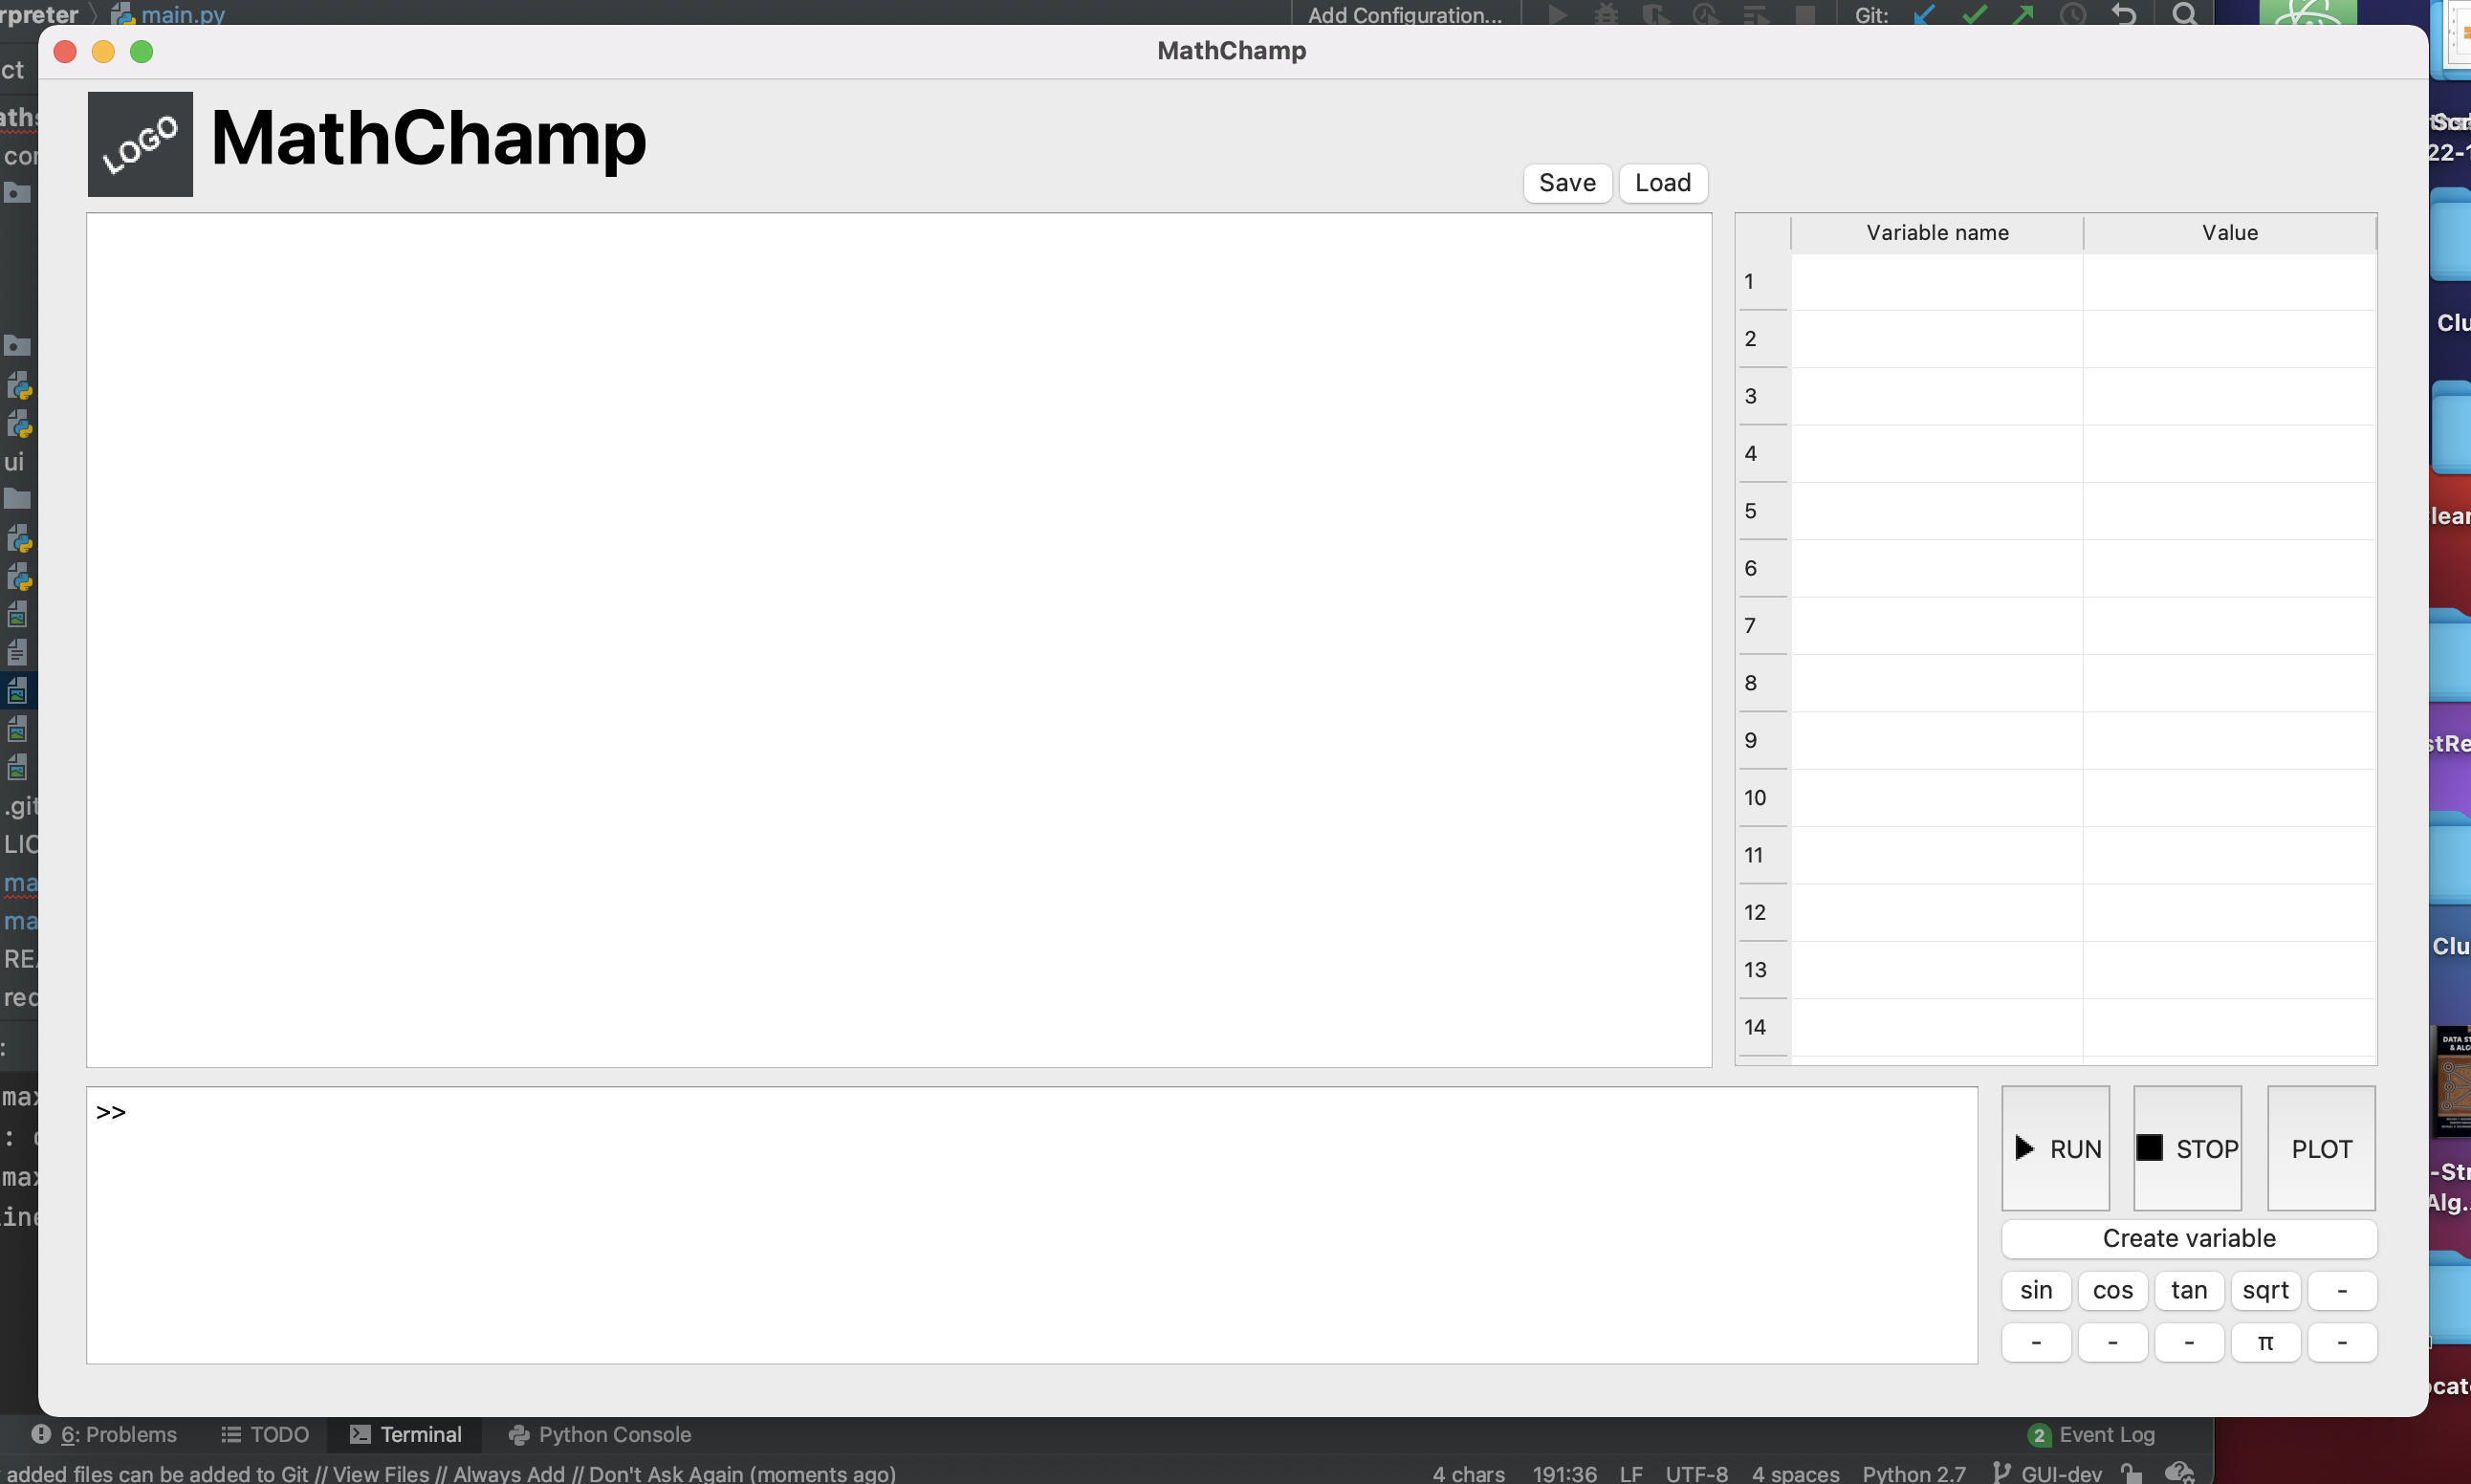
\includegraphics[width=12cm]{2nd_screenshot.png}
    \caption{2nd iteration of GUI from Sprint 3 (13/11/2022)}
    \label{fig:2ndGUI}
\end{figure}

Users can now enter expressions, statements, and commands from the interpreter directly from the intuitive GUI. The GUI was able to be developed quickly as meetings were held amongst the team to collaboratively create a lo-fi and medium-fi prototype of the GUI as evidence in Appendix \ref{designs}. Since last week, there has been the addition of being able to save, and load scripts at the top corner. Once the user presses 'run' add the commands within the script will run in succession; alternatively you could just run a section of the script by highlighting those commands. Using the 'Create Variable' button, users are prompted with the Create Variable window where they can enter the name and value; which will later be constrained with an error message using ReGEX to do data validation. Created variables will then be shown within a symbols table on the right side of the screen (above the function buttons).

\begin{figure}[h]
    \centering
    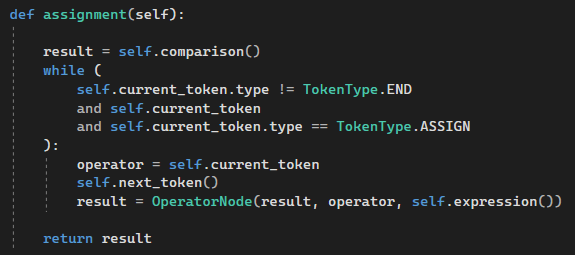
\includegraphics[width=13.0cm]{variableAssignment.png}
    \caption{Syntax Analyser - Variable Assignment (syntaxAnalyzer.py)}
    \label{fig:bnf}
\end{figure}

\subsection{Sprint 4 (14/11/2022)}
In Sprint 4, the focus is on implementing plotting into MathChamp to visualise functions of variables and expressions. The plots will allow users to zoom in and out, alter the subplot configurations, edit axis and curve parameters, reset their view following alterations (with a home button), and to save the plot or custom plot view. Once plotting is functional, Zero Crossings functionality will be looked into. For further additional functionality, development on including Boolean Operators such as Less Than and Greater Than will be started, utilising the following new tokens:

\begin{itemize}
    \item GT = \textit{"GREATER\_THAN"}
    \item LT = \textit{"LESS\_THAN"}
\end{itemize}

Further functions (which are yet to be confirmed) will also explored at this stage of development; there is a prospect for operations on matrices and factorials. The deadline for completion of plotting and Boolean Operators will be set as the 21st of November, 2022.

\begin{figure}[h]
    \centering
    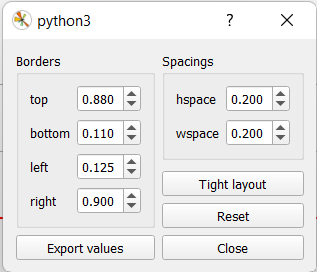
\includegraphics[width=7.0cm]{plottingSubPlots.png}
    \caption{Plotting - General Configuration Options}
    \label{fig:bnf}
\end{figure}

\begin{figure}[h!]
    \centering
    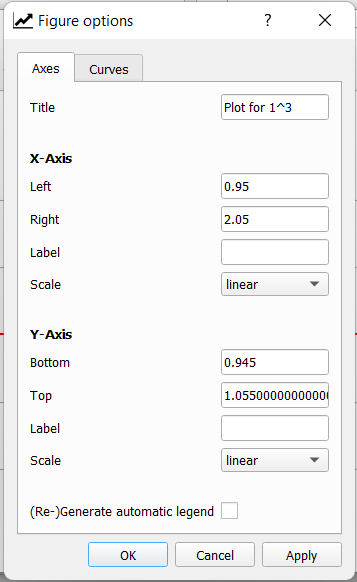
\includegraphics[width=7.0cm]{plottingParameters1.png}
    \caption{Plotting - Subplot Configuration Options (Axes)}
    \label{fig:bnf}
\end{figure}

\begin{figure}[h!]
    \centering
    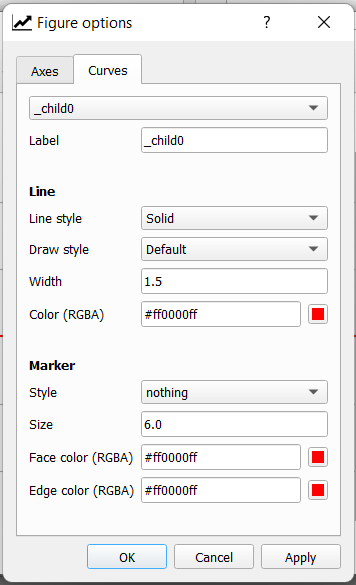
\includegraphics[width=7.0cm]{plottingParameters2.png}
    \caption{Plotting - Subplot Configuration Options (Curves)}
    \label{fig:bnf}
\end{figure}
\FloatBarrier

The plotting was done using our interpreter, and using the output of the interpreter to popular \emph{Python} lists which then correspond to the x and y axis of the plot. The interval the user inputs populates a list corresponding to the x axis, and then the 'x' within the function is substituted by the values in the aforementioned x-axis list to be executed through the interpreter and populate  y-axis list. This is also the sprint where variable dependency functionality was successfully added to our software. This is further explained and explored within \ref{variable-dep-sec}.

\begin{figure}[h!]
    \centering
    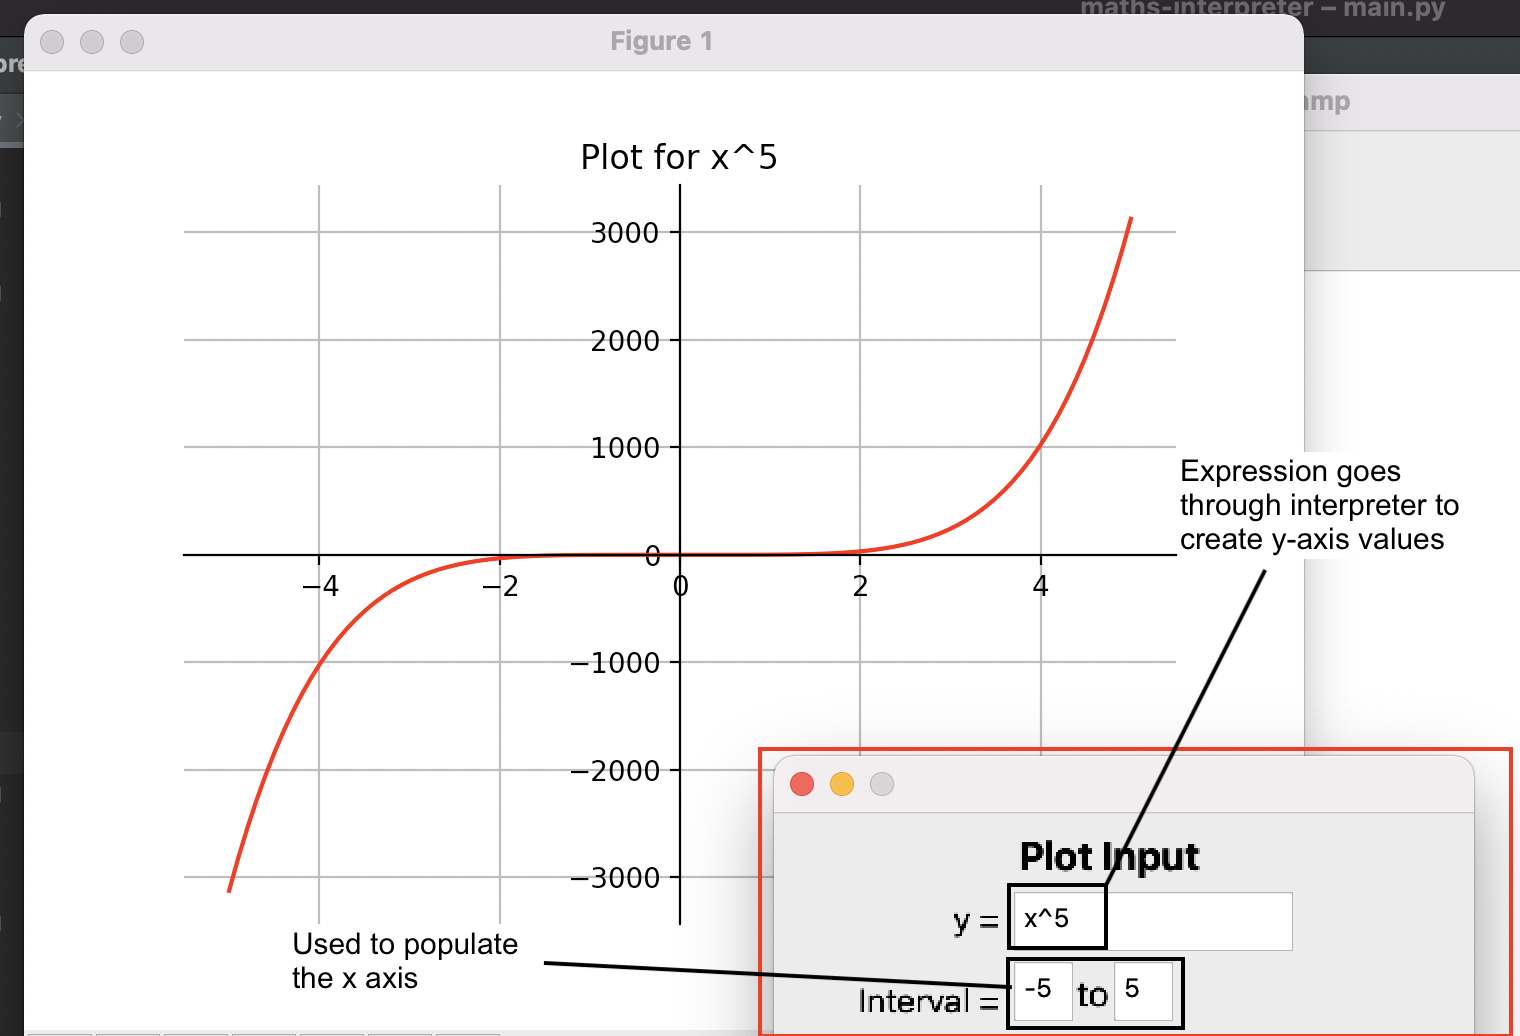
\includegraphics[width=11cm]{plot.png}
    \caption{Example plot}
    \label{fig:plot}
\end{figure}
\FloatBarrier

\newpage
\section{Final implementation}

In terms of functionality and appearance, the GUI is completely finished. The only changes that will need to be changed will be ones in response to changes to the interpreter (such changing the function buttons in response to what functions are included and omitted due to changing scope). 

\begin{figure}[H]
    \centering
    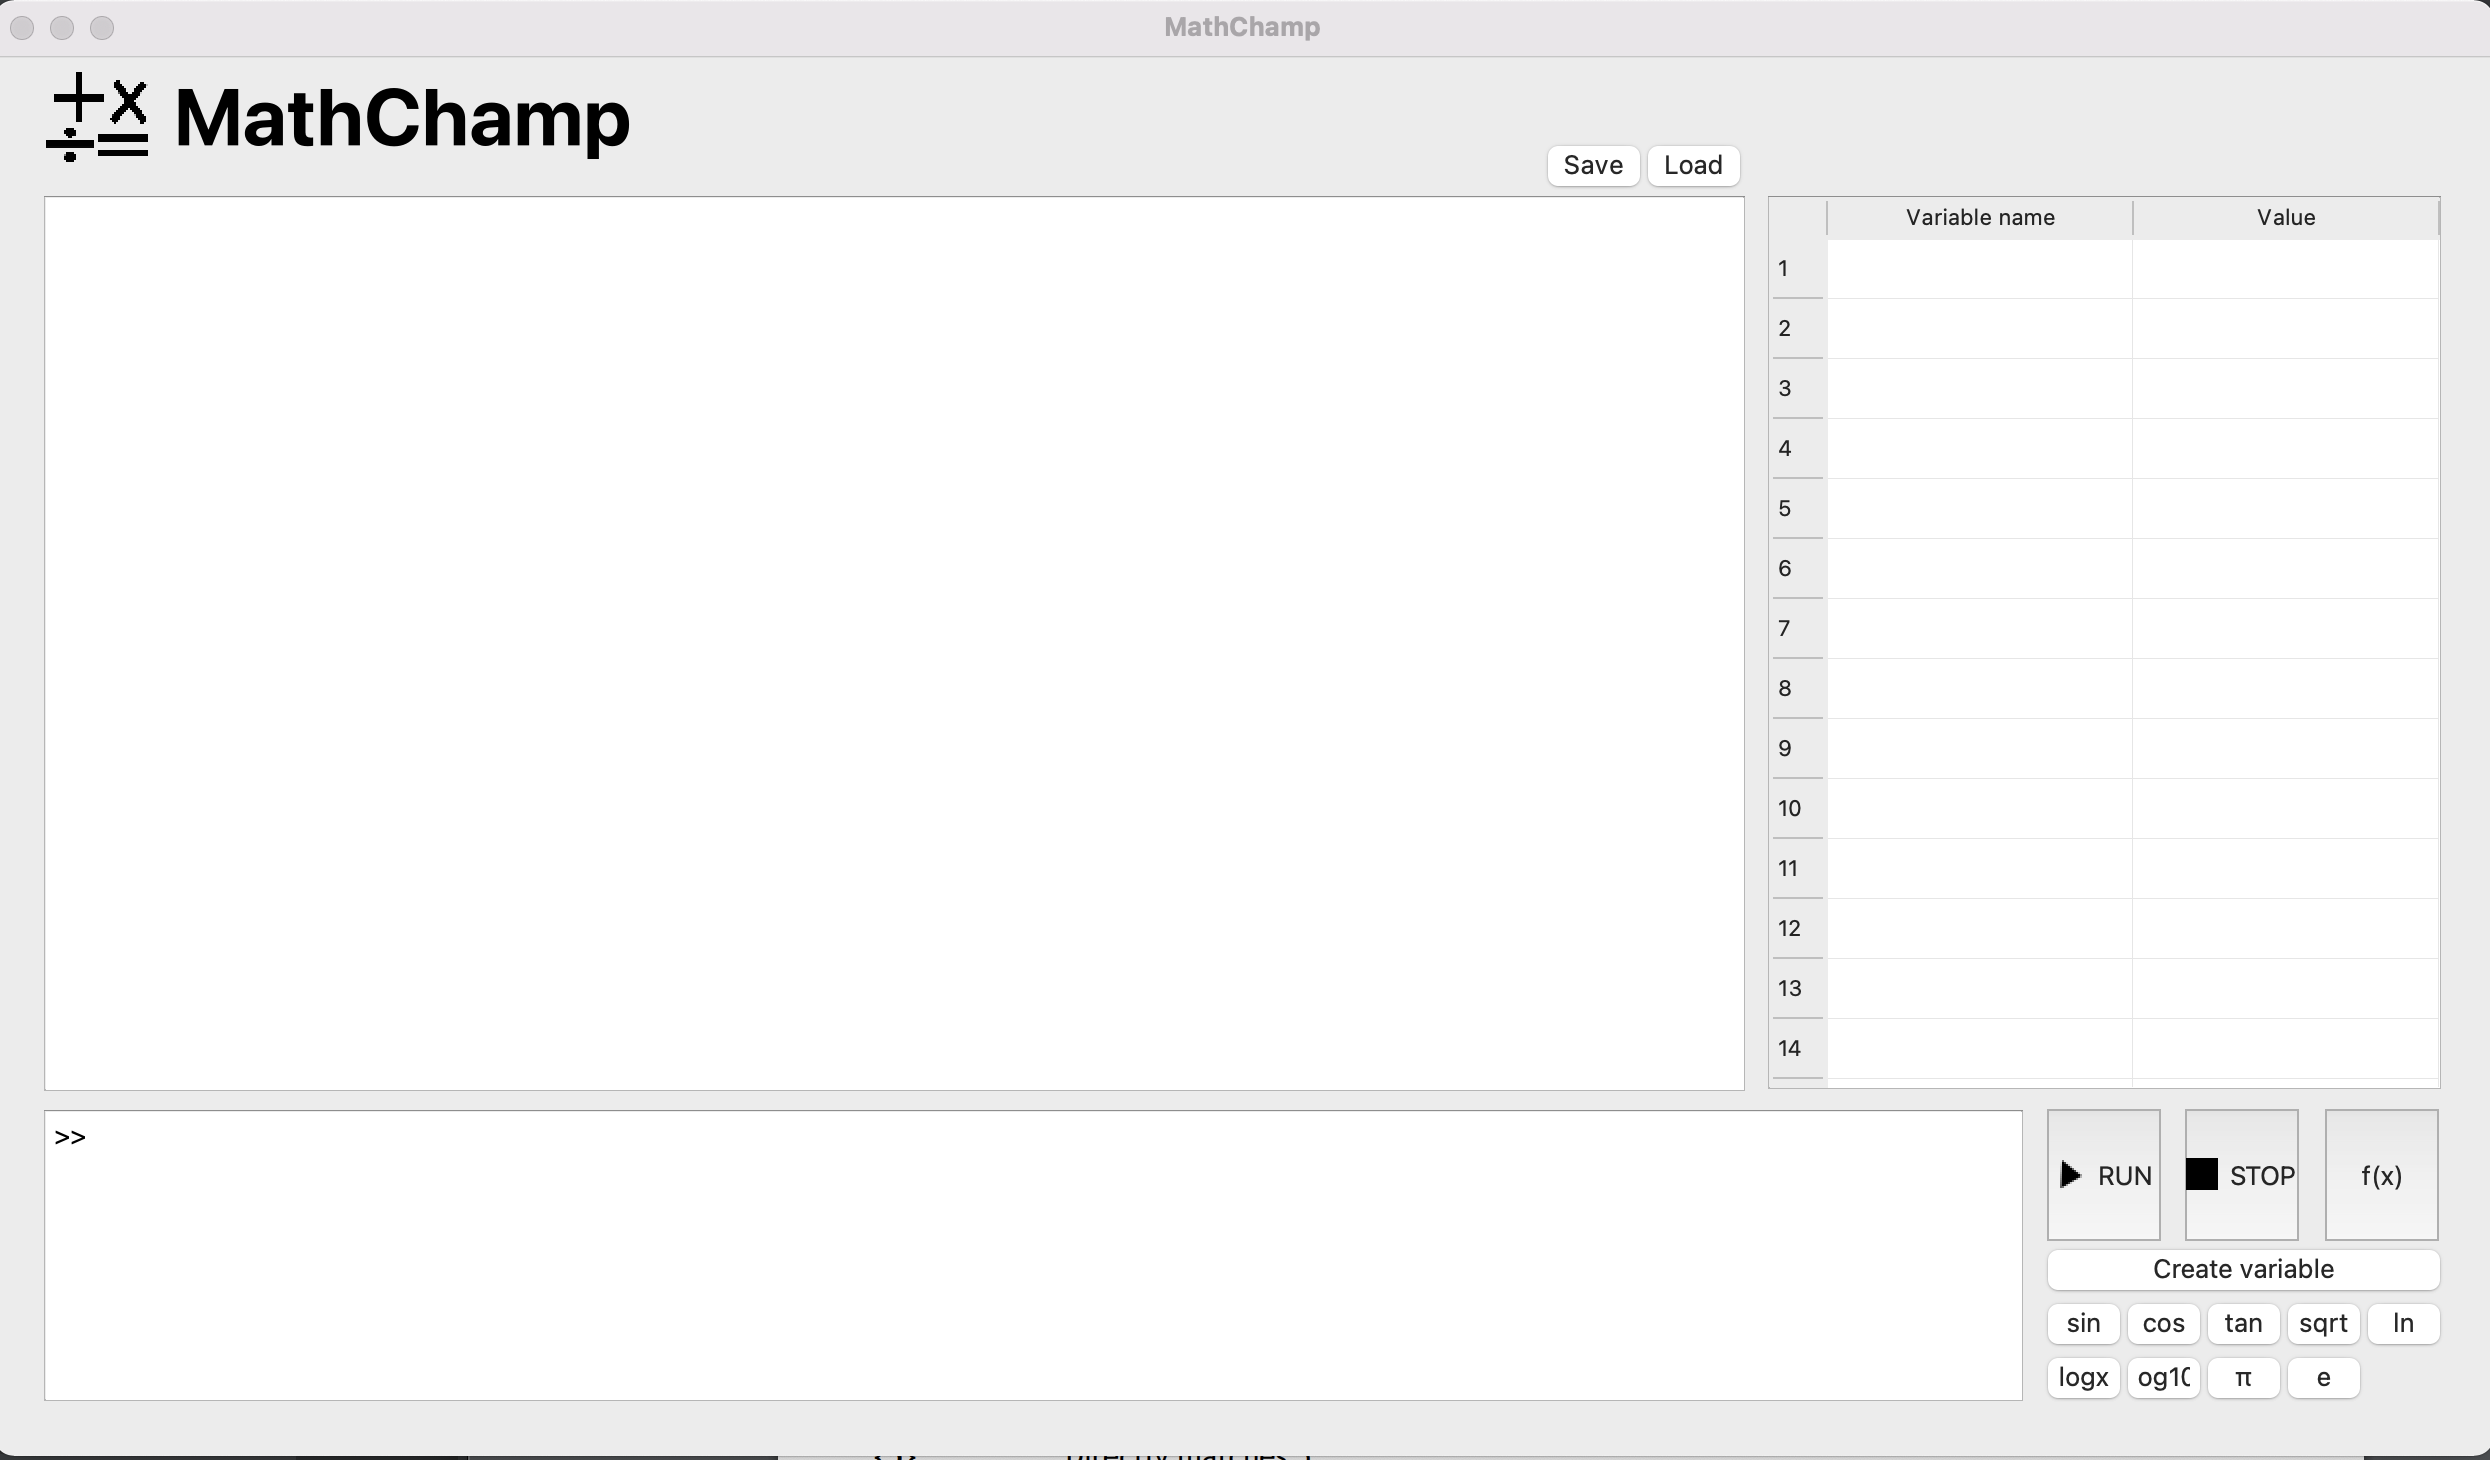
\includegraphics[width=13cm]{3rd_screenshot.png}
    \caption{3rd iteration of GUI}
    \label{fig:3rdGUI}
\end{figure}

\textbf{29/11/2022} \\

Factorials were successfully implemented into the code, through iteration during development. Originally, factorial was implemented through regular mathematical notation (such as \emph{10!}) and was working correctly. However, as the implementation of functions was added to the software it made more sense to implement factorials as a function such as "fact(10)". Therefore, this is how factorials are done in the final program. 

While the GUI was finished from a functionality view point, there was one problem that was left unaddressed. The GUI was developed using a \emph{Mac}, which meant that which the application worked functionally on all machines; some of the spacing between elements wasn't correct (demonstrated in \ref{fig:overlap}) and the text size was too large (\ref{fig:textsize}). However, this was easily fixed by simply setting the style sheet within the program so there's uniformity between all operating systems. 

\begin{figure}[H]
    \centering
    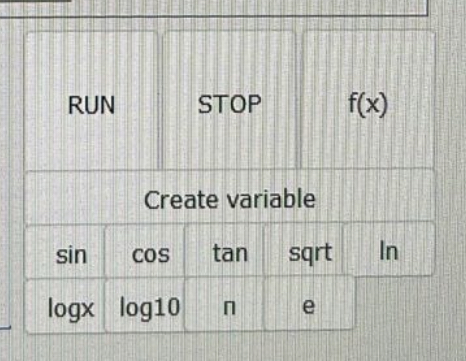
\includegraphics[width=8cm]{development_issues1.jpg}
    \caption{Overlapping elements on Windows}
    \label{fig:overlap}
\end{figure}

\begin{figure}[H]
    \centering
    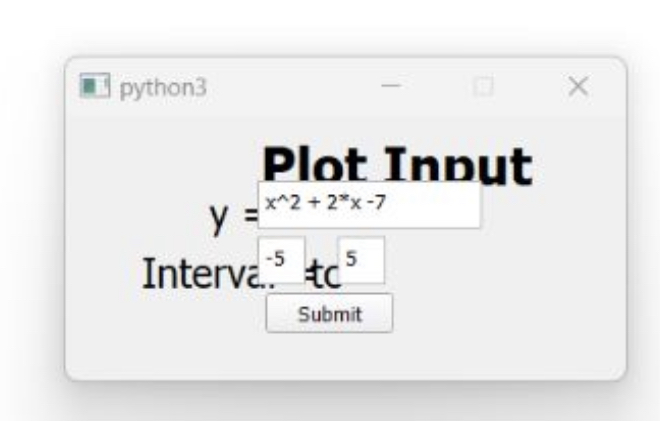
\includegraphics[width=8cm]{development_issues2.jpg}
    \caption{Incorrect text size on Windows}
    \label{fig:textsize}
\end{figure}

Additionally, zero crossings were implemented into our system. This is done by having a parameter on the plot input window which determines the interval for zero crossing which then displays as text in the top-corner of the graph. This is further explored in section \ref{zero-crossing-sec}.

Furthermore, functions such as SIN, COS, TAN, and FACT were also prioritised during our final sprint. Initially issues were faced with the order of precedence, but the issue was identified and resolved the bug. Following the implementation and testing of these functions, Zero Crossings was refined and tested against the new functionalities. The final actions in this implementation stage included increasing the code efficiency, improving and adding further comments, and final testing.

\newpage

\begin{figure}[H]
    \centering
    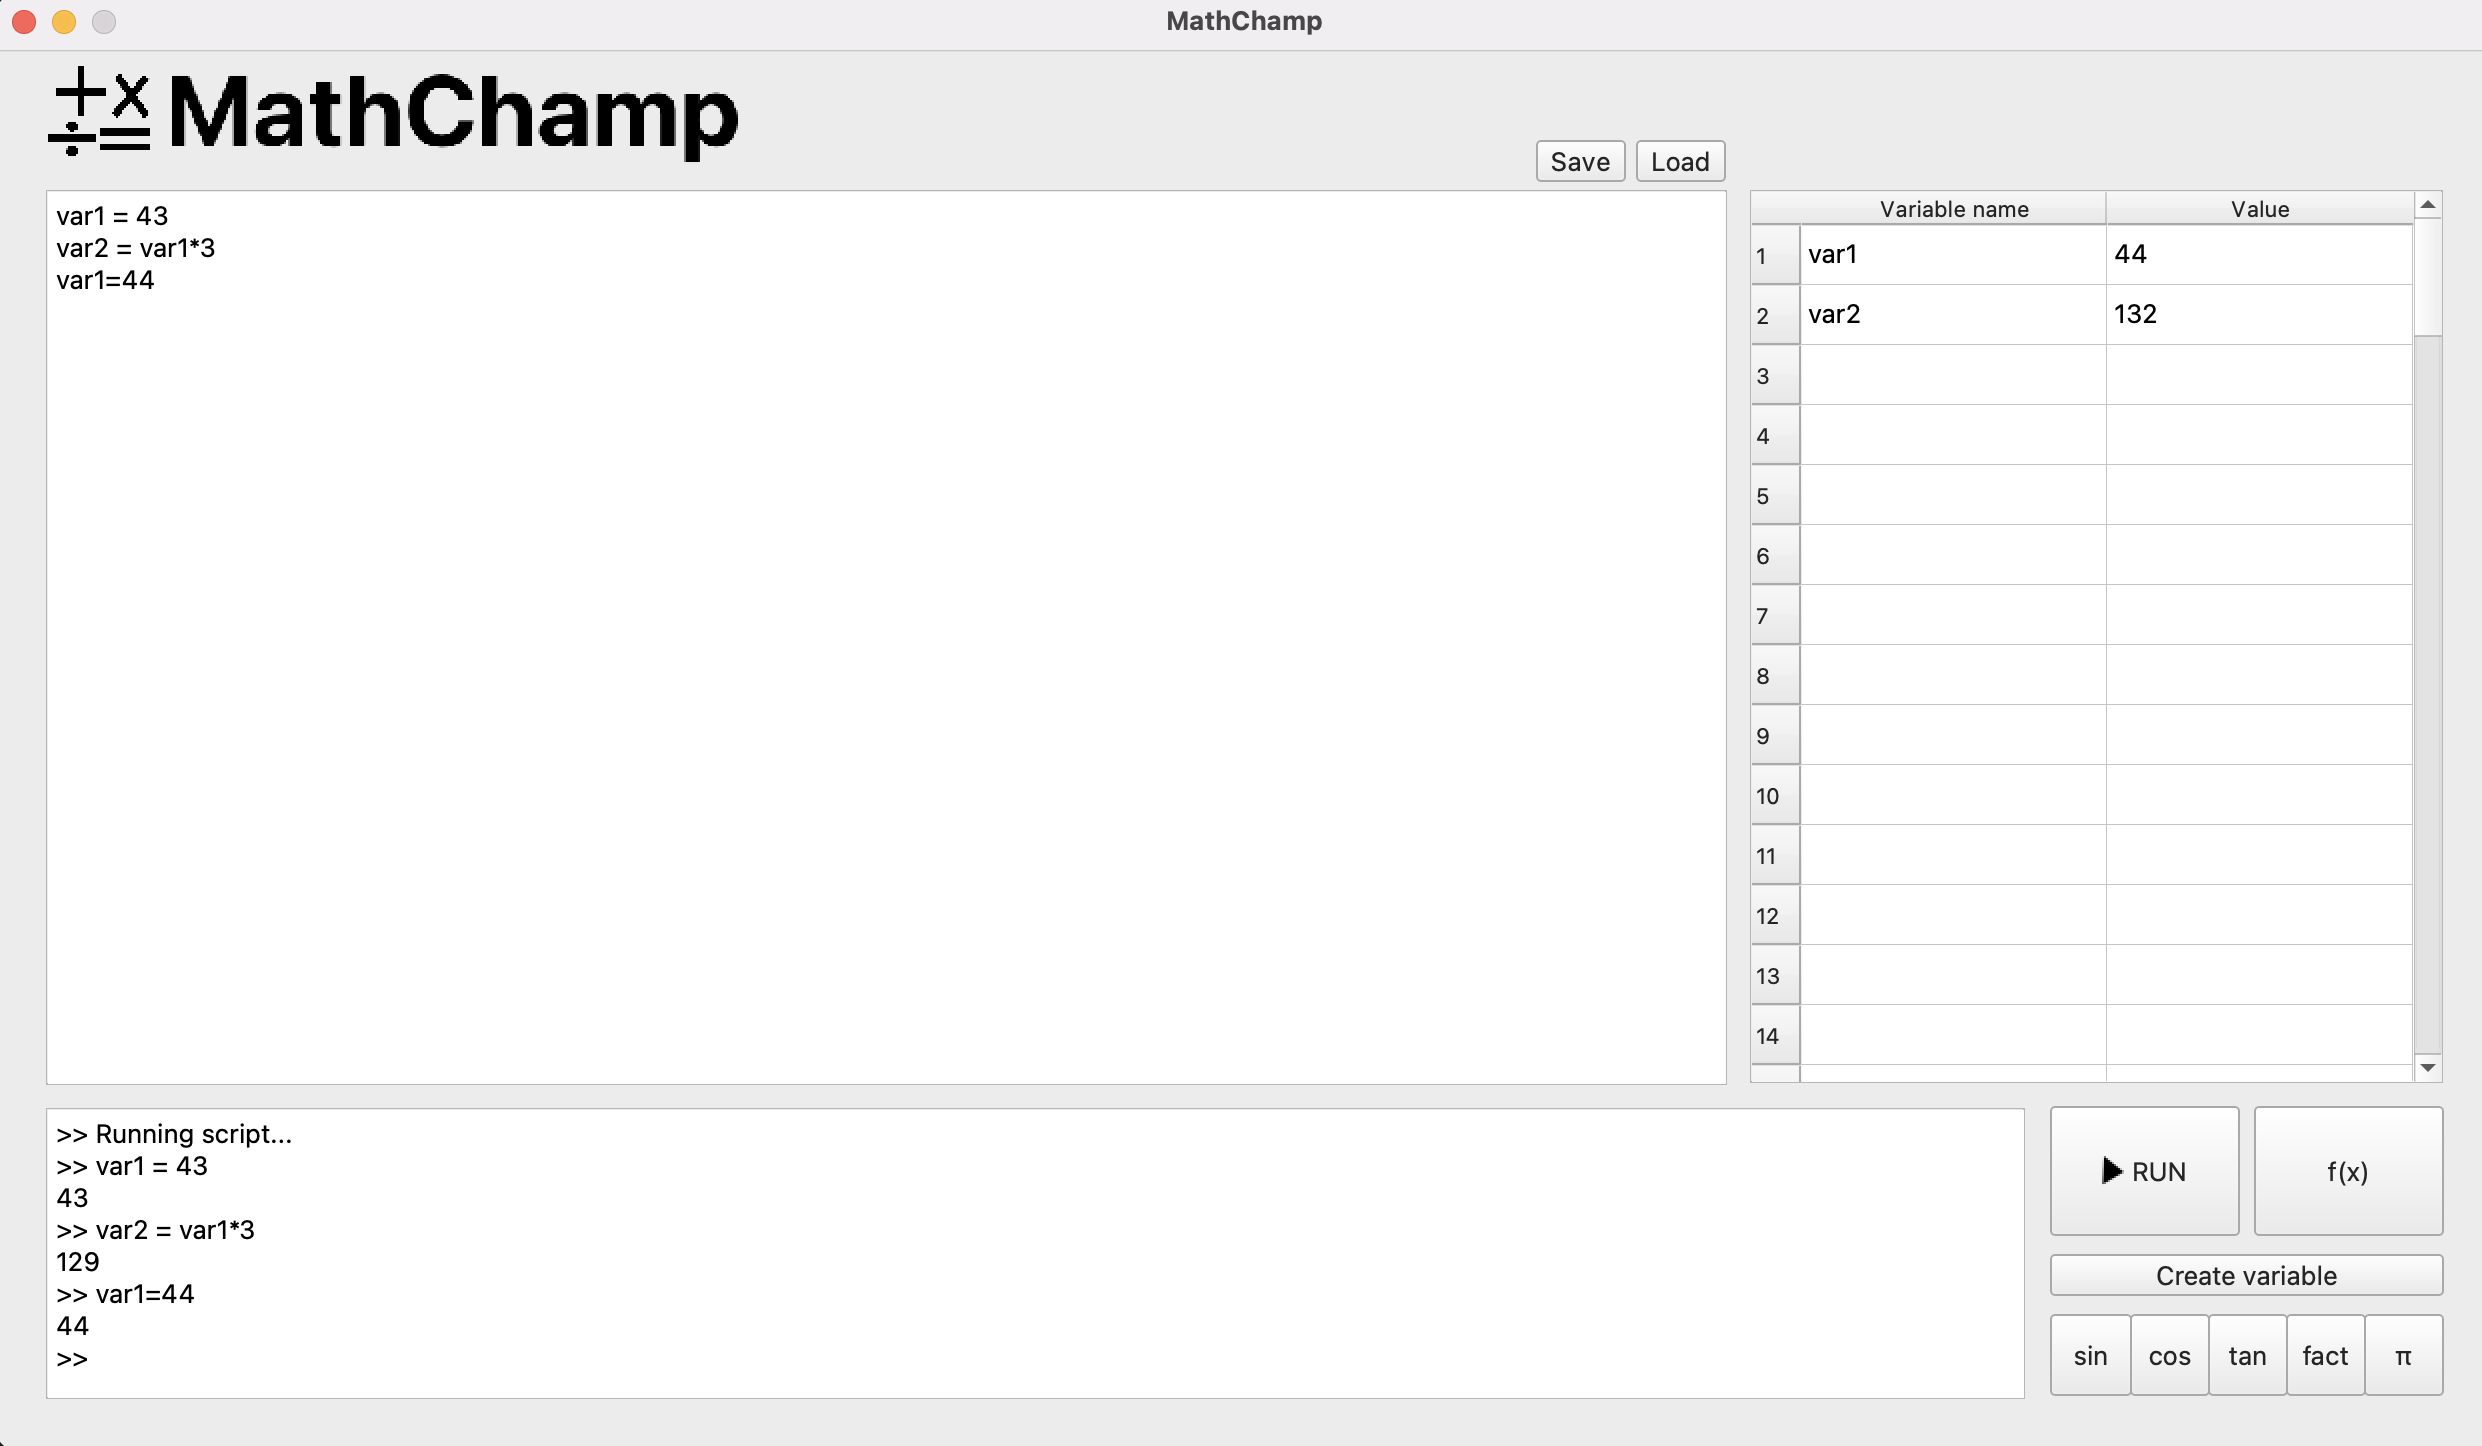
\includegraphics[width=15cm]{final_main.jpg}
    \caption{Final main window}
    \label{fig:final_main}
\end{figure}

\begin{figure}[H]
    \centering
    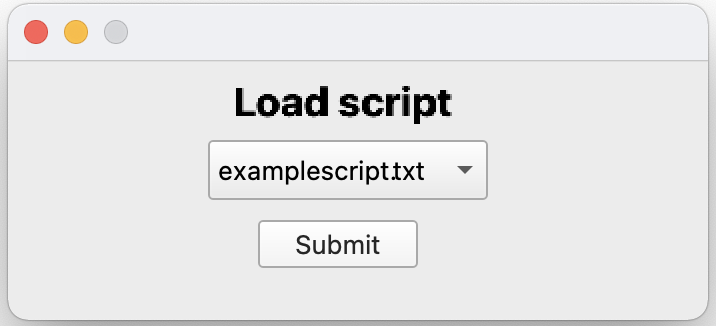
\includegraphics[width=7cm]{final_load.jpg}
    \caption{Final load window}
    \label{fig:final_load}
\end{figure}

\begin{figure}[H]
    \centering
    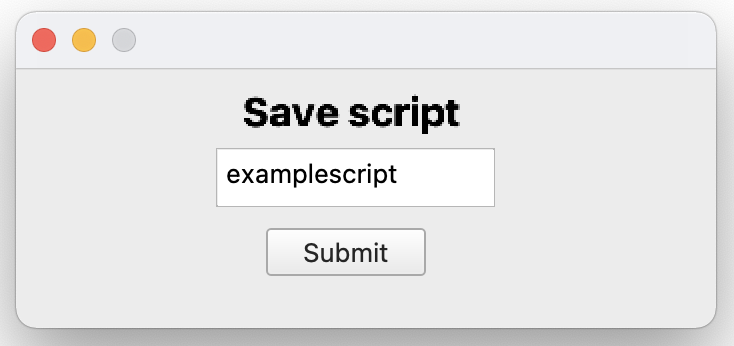
\includegraphics[width=7cm]{final_save.jpg}
    \caption{Final save window}
    \label{fig:final_save}
\end{figure}

\begin{figure}[H]
    \centering
    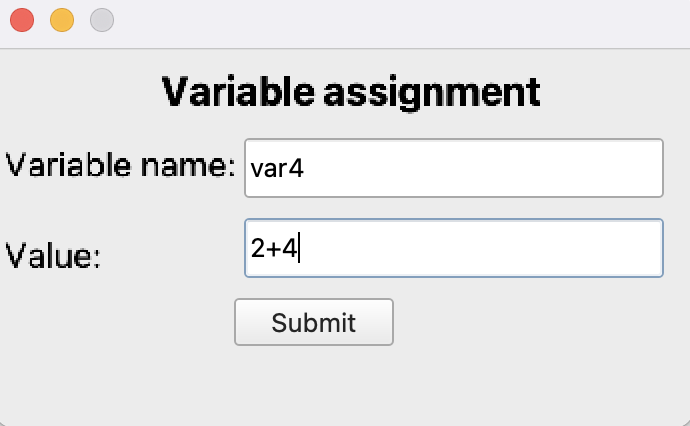
\includegraphics[width=7cm]{final_var.jpg}
    \caption{Final variable window}
    \label{fig:final_variable}
\end{figure}

\begin{figure}[H]
    \centering
    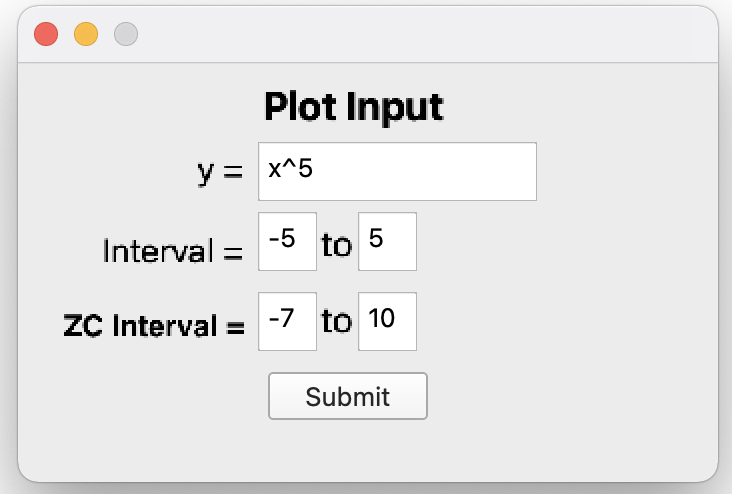
\includegraphics[width=8cm]{final_plotwin.jpg}
    \caption{Final plot input window}
    \label{fig:final_plot_input}
\end{figure}

\begin{figure}[H]
    \centering
    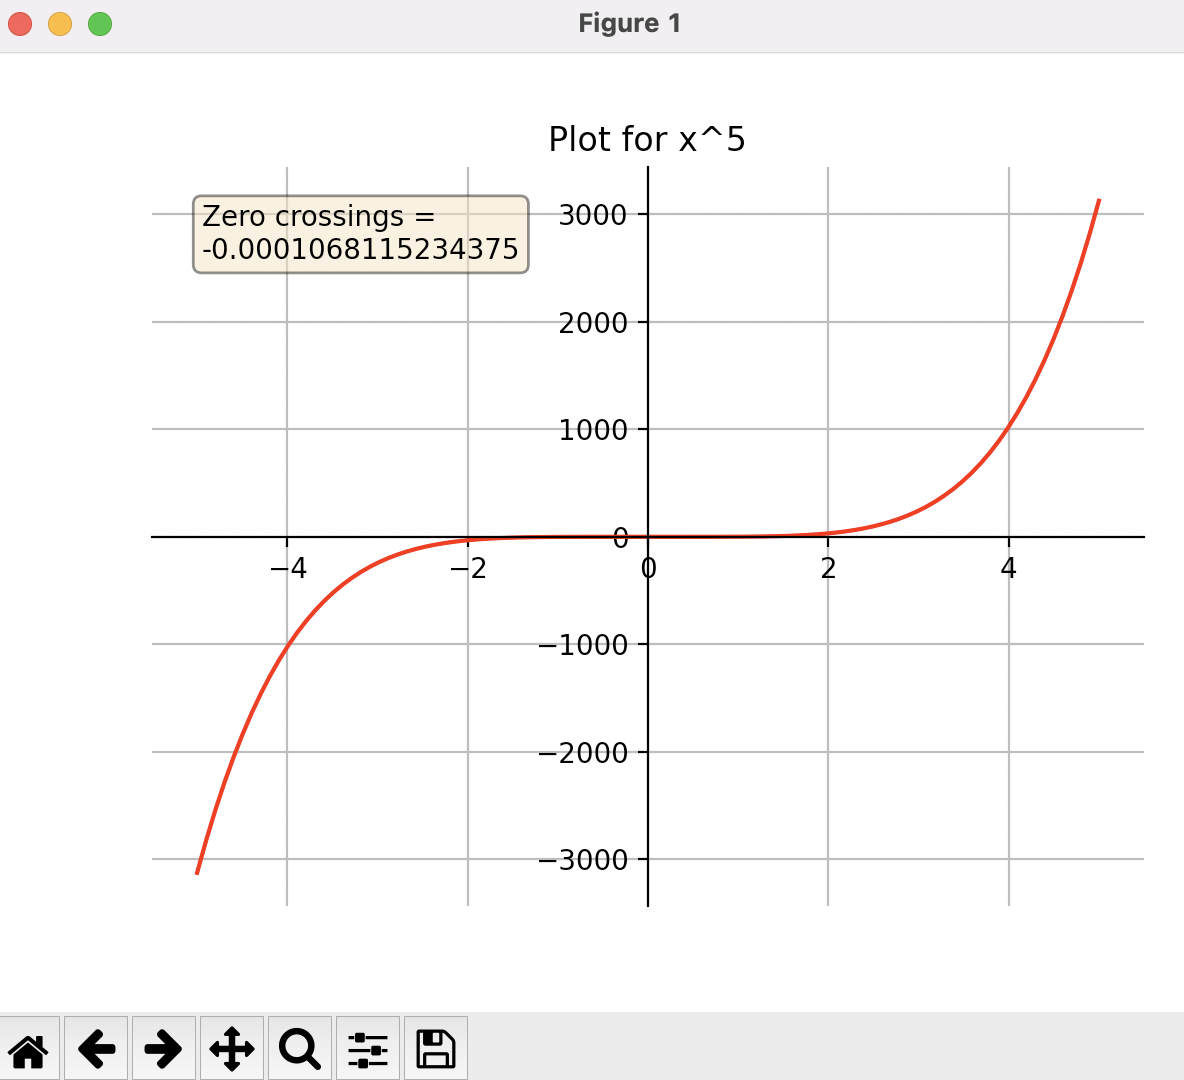
\includegraphics[width=13cm]{final_plot.jpg}
    \caption{Final plot window using Matplotlib}
    \label{fig:final_plot}
\end{figure}

\newpage

\chapter{Testing}\label{Testing}
\section{Manual Test Plan}
The manual test plan are is shown in the appendices at the end of this report; figures \ref{fig:tests1-25}, \ref{fig:tests26-50}, \ref{fig:tests51-75}, \ref{fig:tests76 - 100}. Manual testing was performed at every stage of the development, before the implementation of new code and after. There was a critical focus on ensuring the correct order of precedence to ensure accurate program logic. All aspects of GUI functionality were too tested, including all buttons, plotting, and general system compatibility such as operating system support, window resizing, and input validation.\\\\
\textbf{Note:} MathChamp was tested on \emph{Windows 8.1, 10, 11}, and \emph{MacOS}. The code was written using Windows, and the GUI developed using \emph{MacOS}.


\section{Unit Testing}
The Pytest Framework was incorporated for Unit Testing to ensure complex and efficient functionality testing of the MathChamp Interpreter.

\begin{itemize}
    \item \textbf {Pytest Version:} 7.2.0
    \item \textbf {Platform:} Linux-5.15.0-52-generic-x86\_64-with-glibc2.35
    \item \textbf {Python version:}	3.10.6
    \item \textbf {Packages:} "pluggy": "1.0.0", "pytest": "7.2.0"
    \item \textbf {Plugins:} "html": "3.2.0", "metadata": "2.0.4"
\end{itemize}

Please refer to figures \ref{fig:pytest1}, \ref{fig:pytest2}, and \ref{fig:pytest3} on the pages which follow.

\begin{figure}[H]
    \centering
    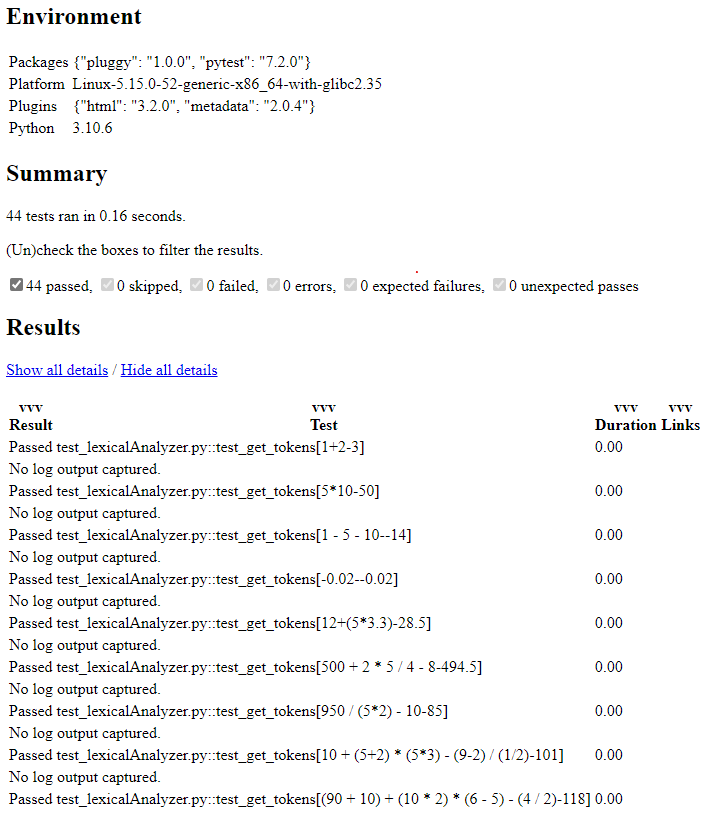
\includegraphics[width=15cm]{pytest 1.png}
    \caption{Test Page 1}
    \label{fig:pytest1}
\end{figure}

\begin{figure}[H]
    \centering
    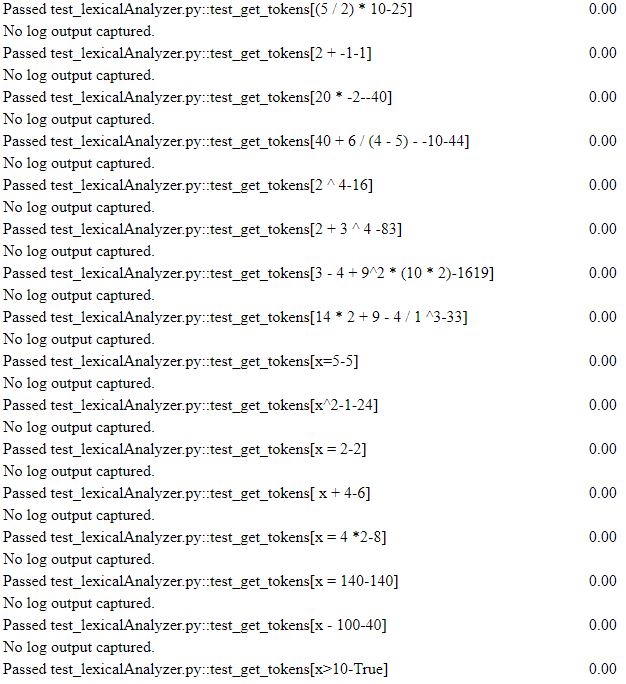
\includegraphics[width=15cm]{pytest 2.png}
    \caption{Test Page 2}
    \label{fig:pytest2}
\end{figure}

\begin{figure}[H]
    \centering
    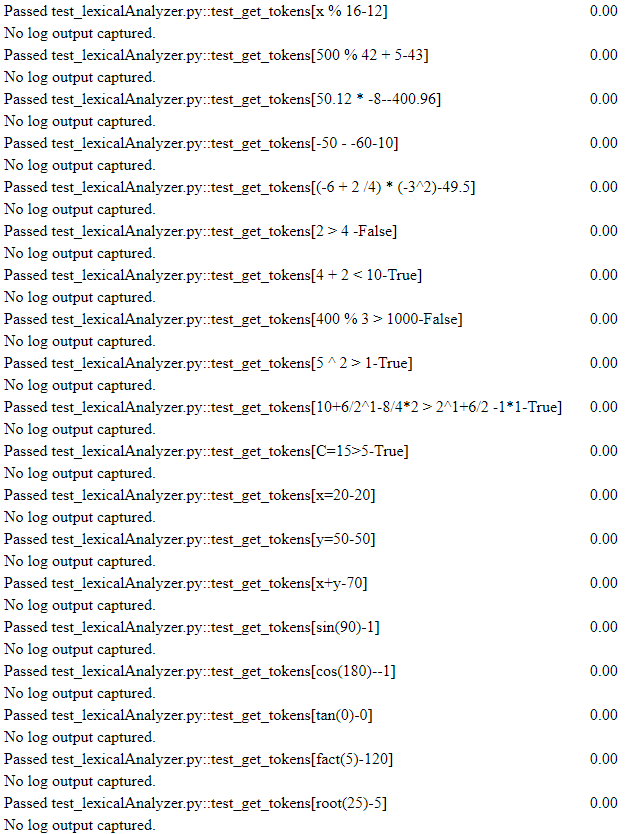
\includegraphics[width=15cm]{pytest 3.png}
    \caption{Test Page 3}
    \label{fig:pytest3}
\end{figure}



\chapter{Discussion, conclusion and future work}\label{Conclusions}

The final MathChamp product meets all of the 'Must Have' and 'Should Have' MoSCoW requirements. It is well-tested, well-documented software with clean code, an intuitive GUI, variable assignment and visualisation, accurate BODMAS order of operations, and visualisation of Mathematical Functions. All basic arithmetic expressions, professional style plotting functions, and configuration settings are supported. Furthermore, additional functionality has been achieved, such as boolean expressions, zero crossings, an excellent user interface, and broad functionality.

Due to time constraints,  a polar curve spirograph was not implemented into the plotting. Complex numbers and differentiation are also unsupported as they did not make it to the final deliverable. The team decided it was better to focus on refining the existing functionality rather than rush extra functionality and risk a reduction in the robustness of the MathChamp product. However there was elements that weren't in our original MoSCoW such as variable dependency, in addition to meeting two of our 'could' requirements being zero crossings and factorials (as a function). The MathChamp interpreter could be improved by incorporating function differentiation and complex numbers. The interpreter could be made more efficient by improving all code efficiency (such as reducing the number of loops).

To conclude, despite a group restructuring one month into the project causing a considerable delay and some internal group difficulties, the development of our mathematical interpreter, MathChamp, has been a resounding success. 



\bibliographystyle{unsrt} \label{bibliography}
\bibliography{mathChampReferences}
\nocite{*}

\chapter*{Contributions}
\textbf{Descriptions and percentage of contribution by team-member:}

\begin{itemize}
    \item Ebin Paul: \%
    \item Christopher Gavey: \%
    \item Max James: \%
    \item Aswin Sasi: \%
    \item Soniya Avarachan: \%
\end{itemize}

\chapter*{Appendix A}

\section{Design}\label{designs}
\subsection{Lo-Fi Design}

\begin{figure}[h]
    \centering
    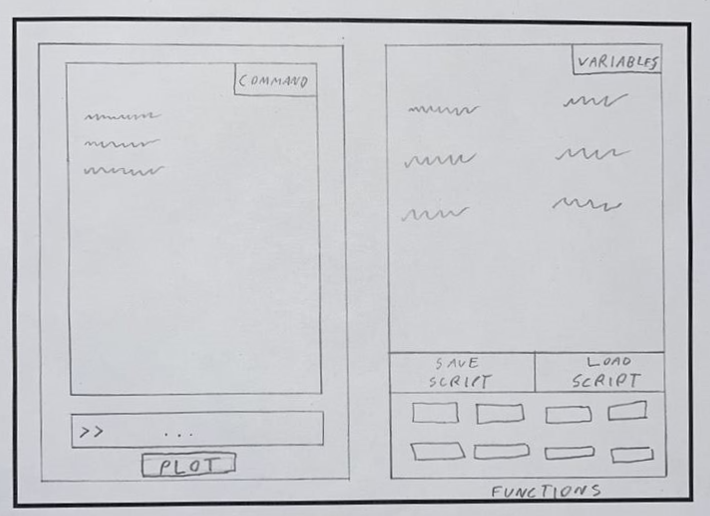
\includegraphics[width=14cm]{LoFiMain.png}
    \caption{Main MathChamp window}
    \label{fig:Lofi-Main}
\end{figure}

\begin{figure}[h]
    \centering
    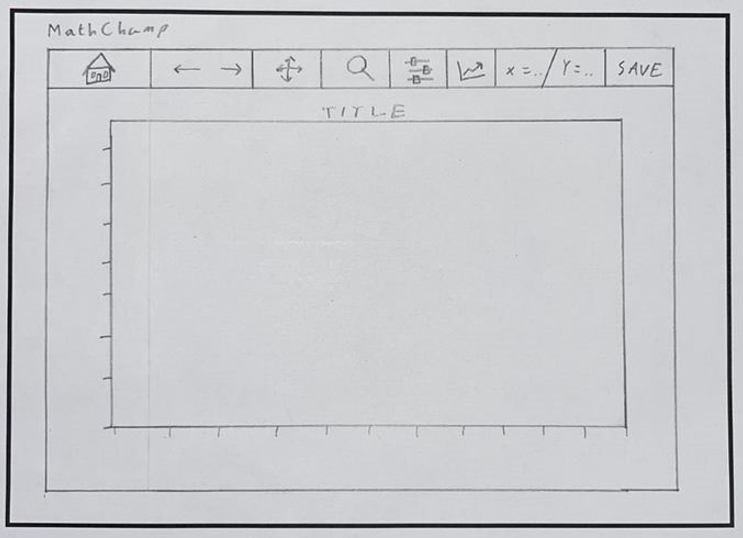
\includegraphics[width=14cm]{LoFiPlot.png}
    \caption{MathChamp plotting window}
    \label{fig:Lofi-Plotting}
\end{figure}

\begin{figure}[h]
    \centering
    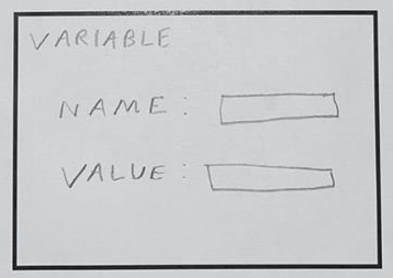
\includegraphics[width=8cm]{LoFiVariable.png}
    \caption{MathChamp variable assignment window}
    \label{fig:Lofi-VariableAssignment}
\end{figure}

\begin{figure}[h]
    \centering
    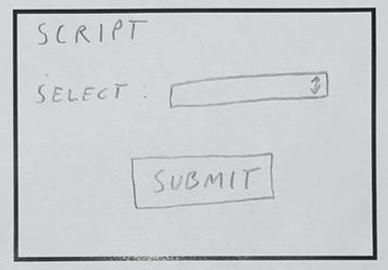
\includegraphics[width=8cm]{loFiScript.png}
    \caption{MathChamp scripts window}
    \label{fig:Lofi-Scripts}
\end{figure}

\FloatBarrier


\subsection{Medium-Fi Design}
\begin{figure}[h]
    \centering
    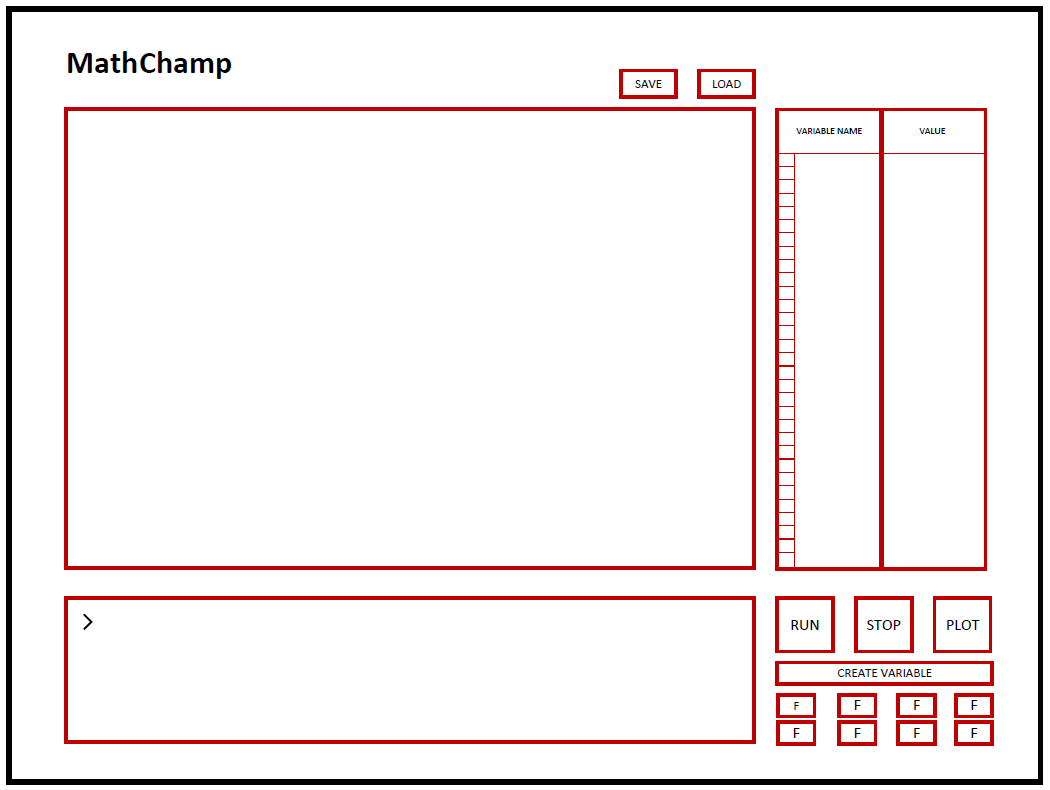
\includegraphics[width=14cm]{MediumFiMain.png}
    \caption{MathChamp main window}
    \label{fig:MediumFi-Main}
\end{figure}

\begin{figure}[h]
    \centering
    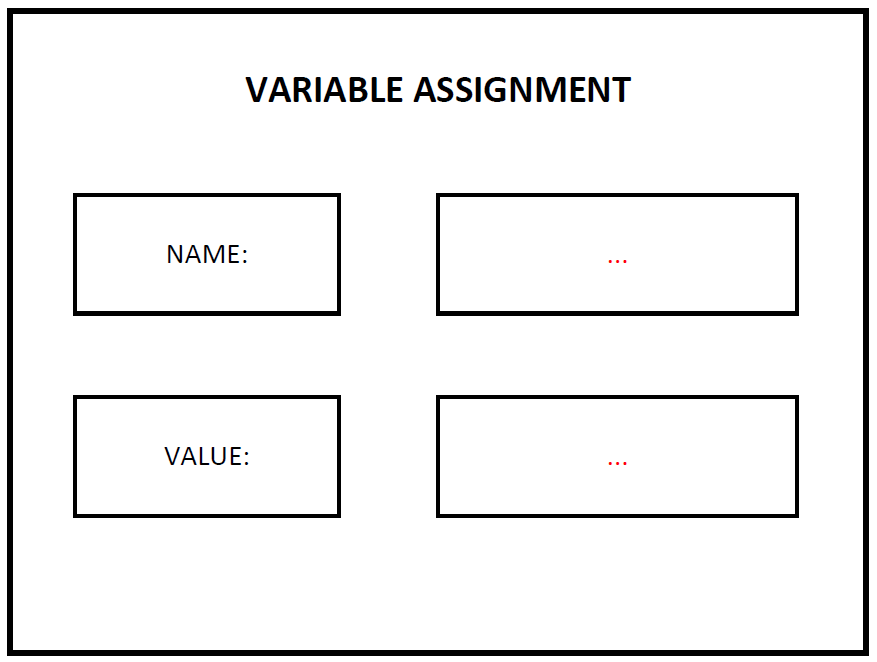
\includegraphics[width=9cm]{MediumFiVariable.png}
    \caption{MathChamp variable assignment window}
    \label{fig:Mediumfi-VariableAssignment}
\end{figure}

\begin{figure}[h]
    \centering
    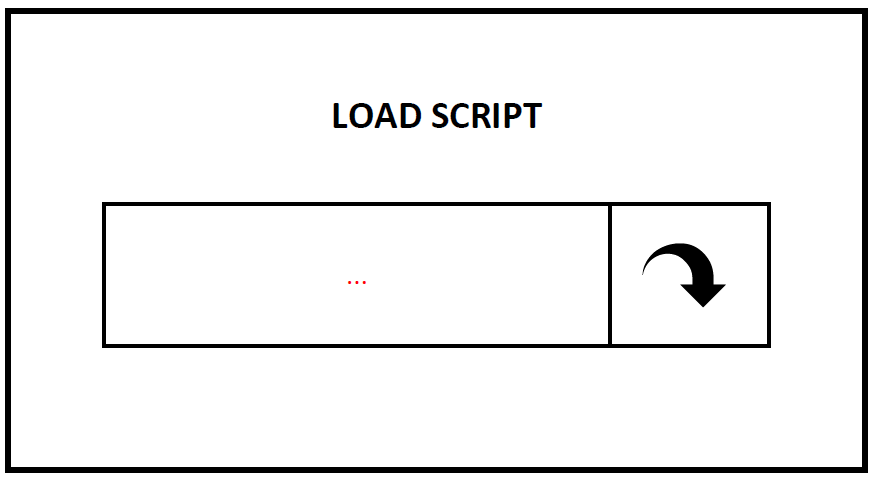
\includegraphics[width=10cm]{MediumFiScript.png}
    \caption{MathChamp scripts window}
    \label{fig:MediumFi-Scripts}
\end{figure}

\begin{figure}[H]
    \centering
    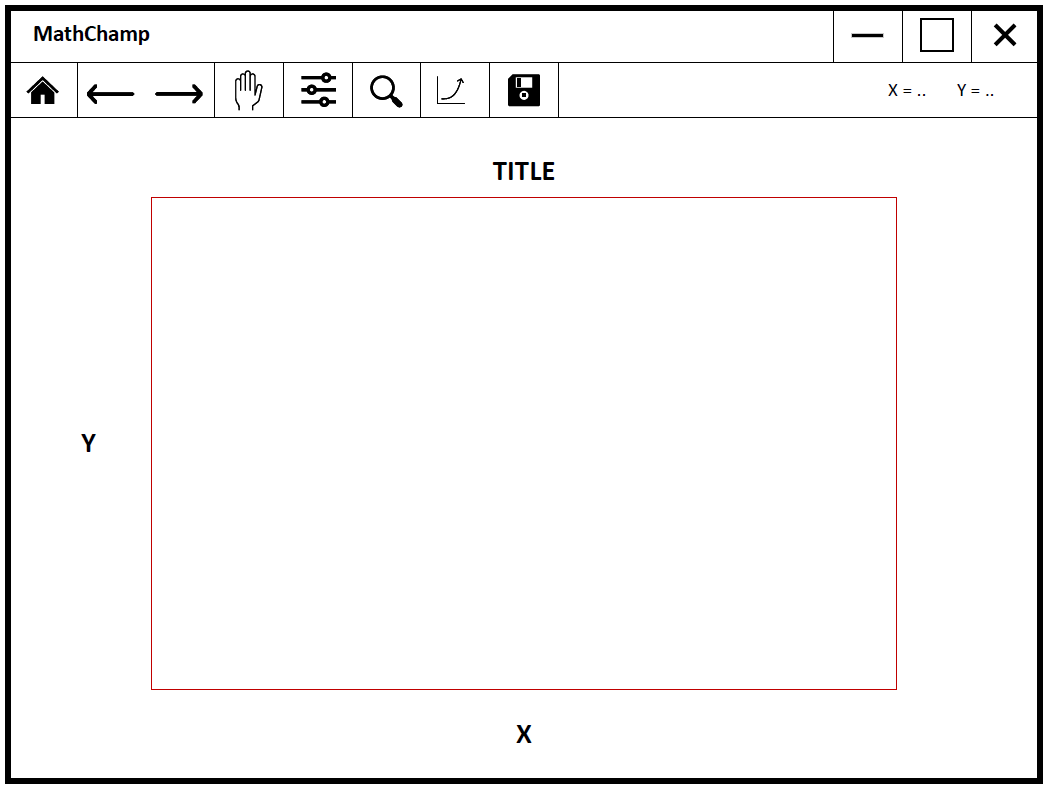
\includegraphics[width=15cm]{MediumFiPlot.png}
    \caption{MathChamp plotting window}
    \label{fig:MediumFi-Plotting}
\end{figure}

\newpage


\section{UML Diagrams}\label{uml-diagrams}

\begin{figure}[H]
    \centering
    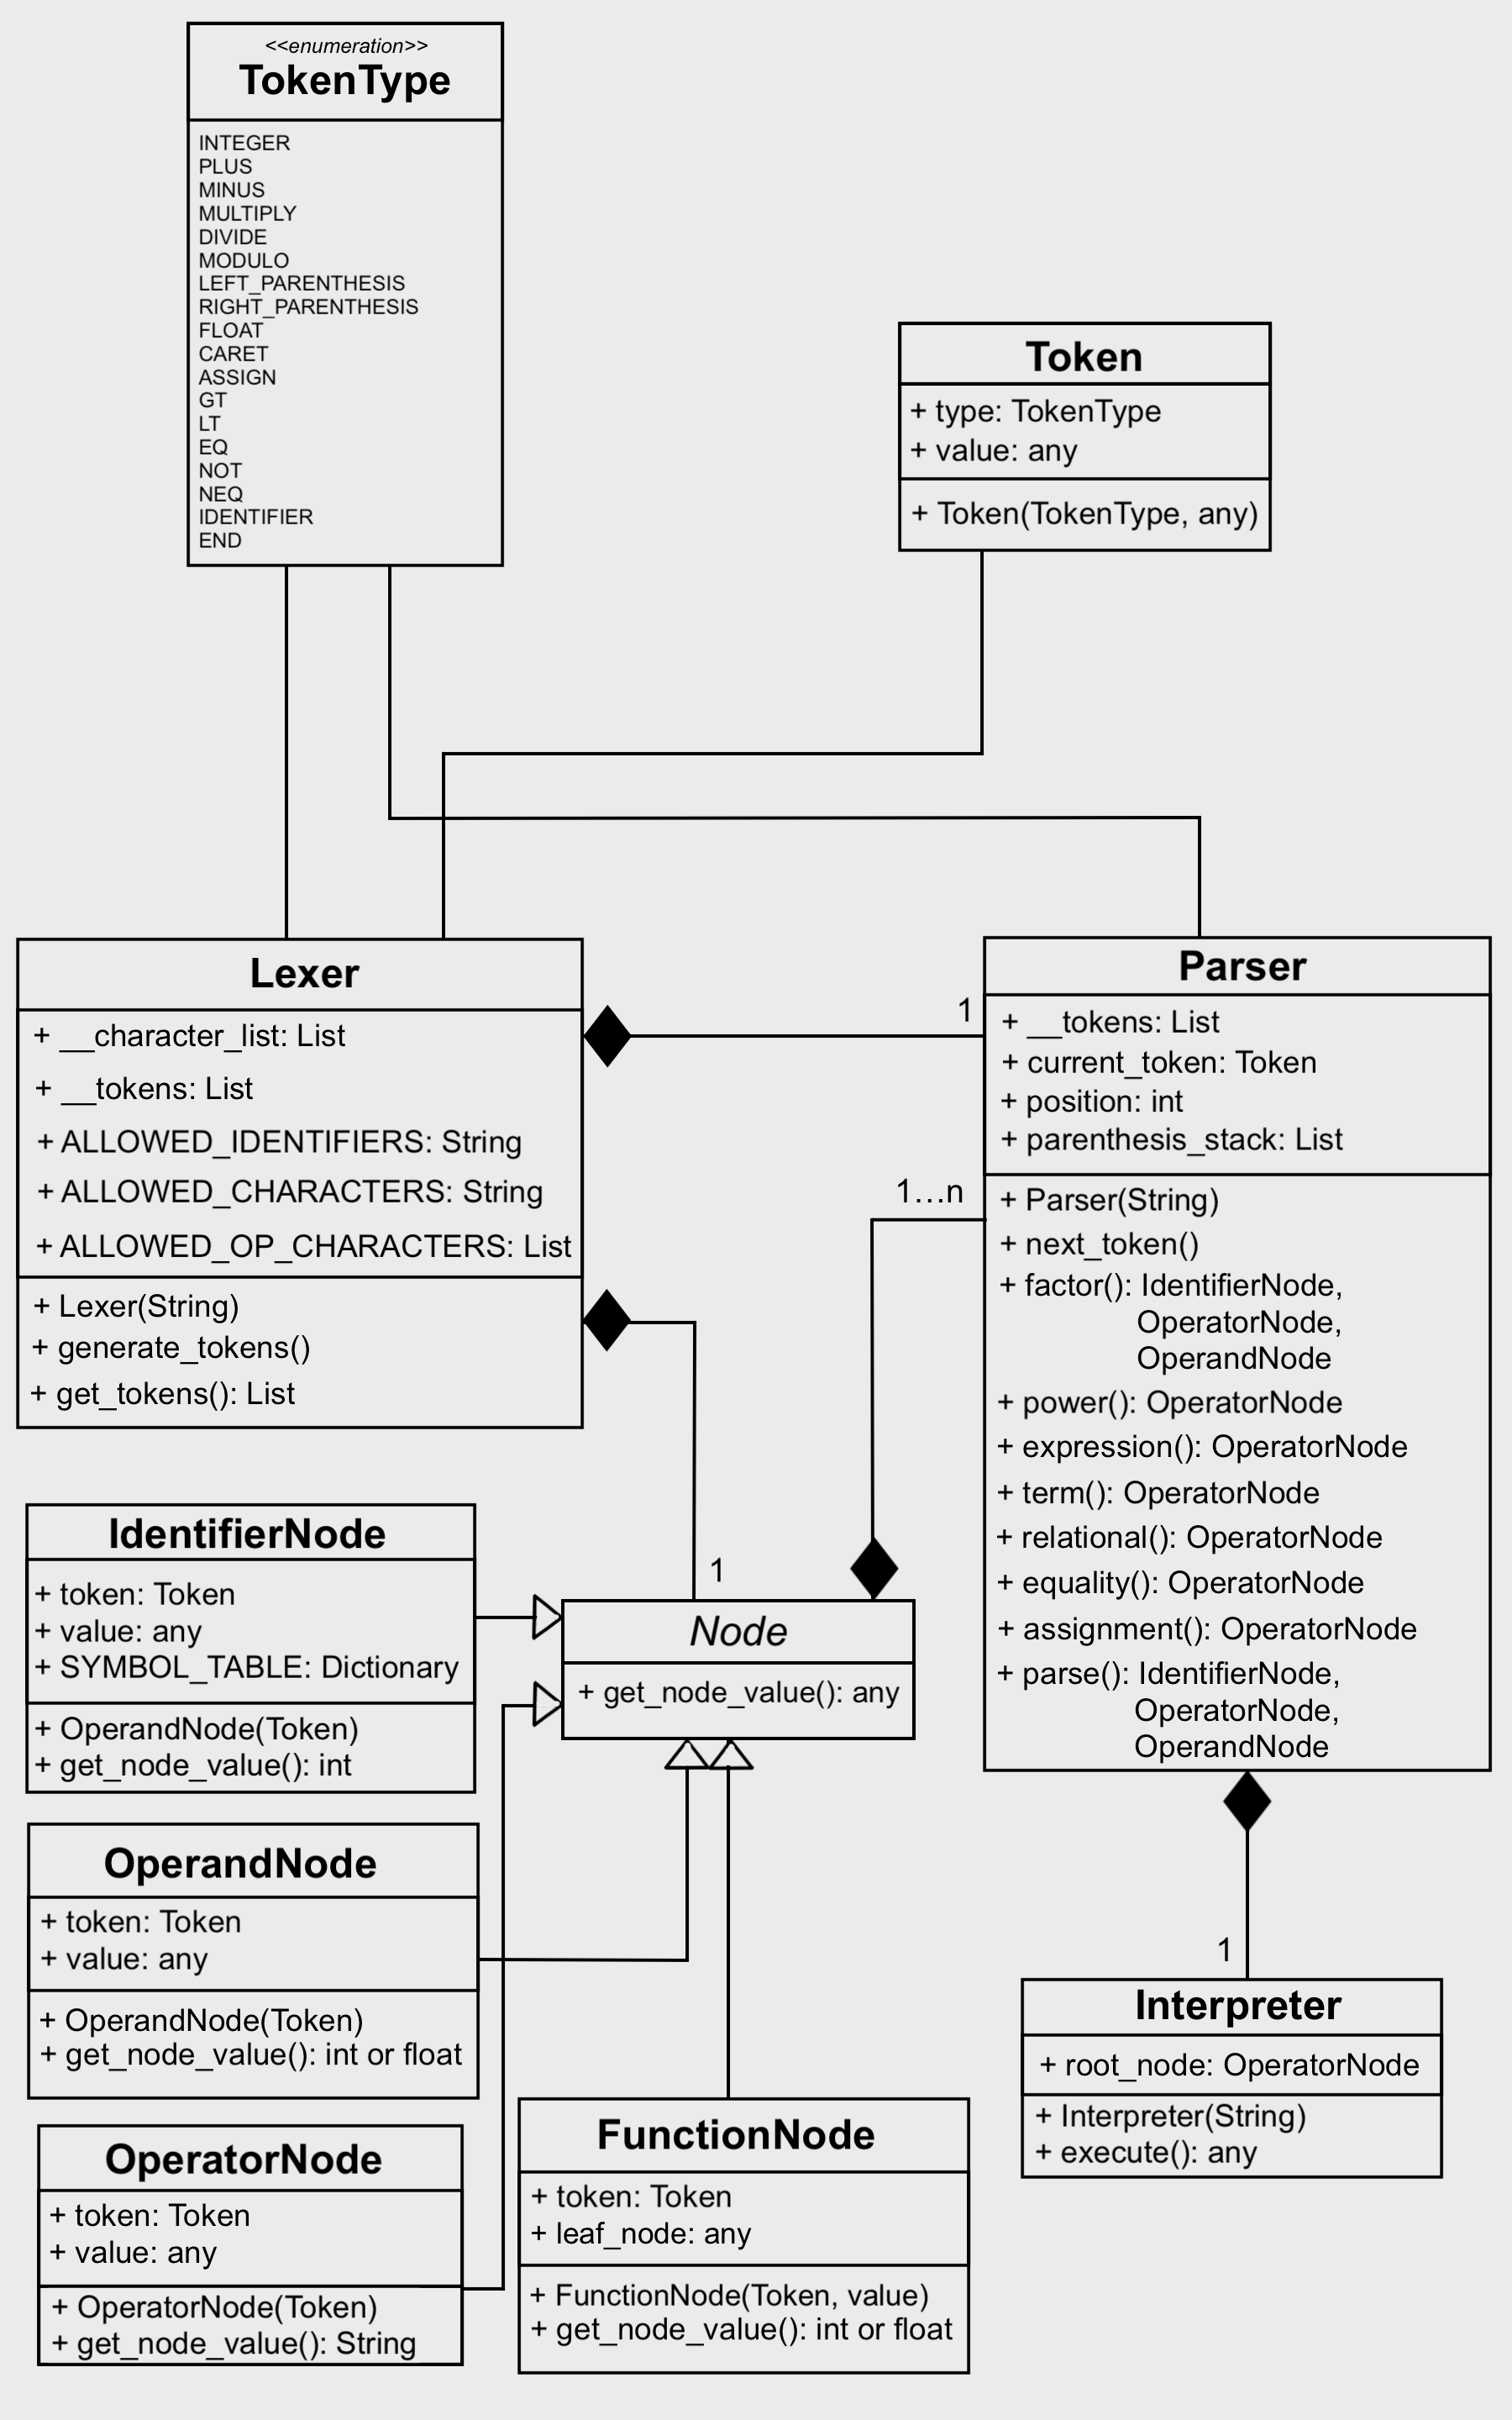
\includegraphics[width=15cm]{UMLClass1.png}
    \caption{UML Class diagram for the Interpreter}
    \label{fig:UMLClassInterpreter}
\end{figure}

\newpage

\begin{figure}[H]
    \centering
    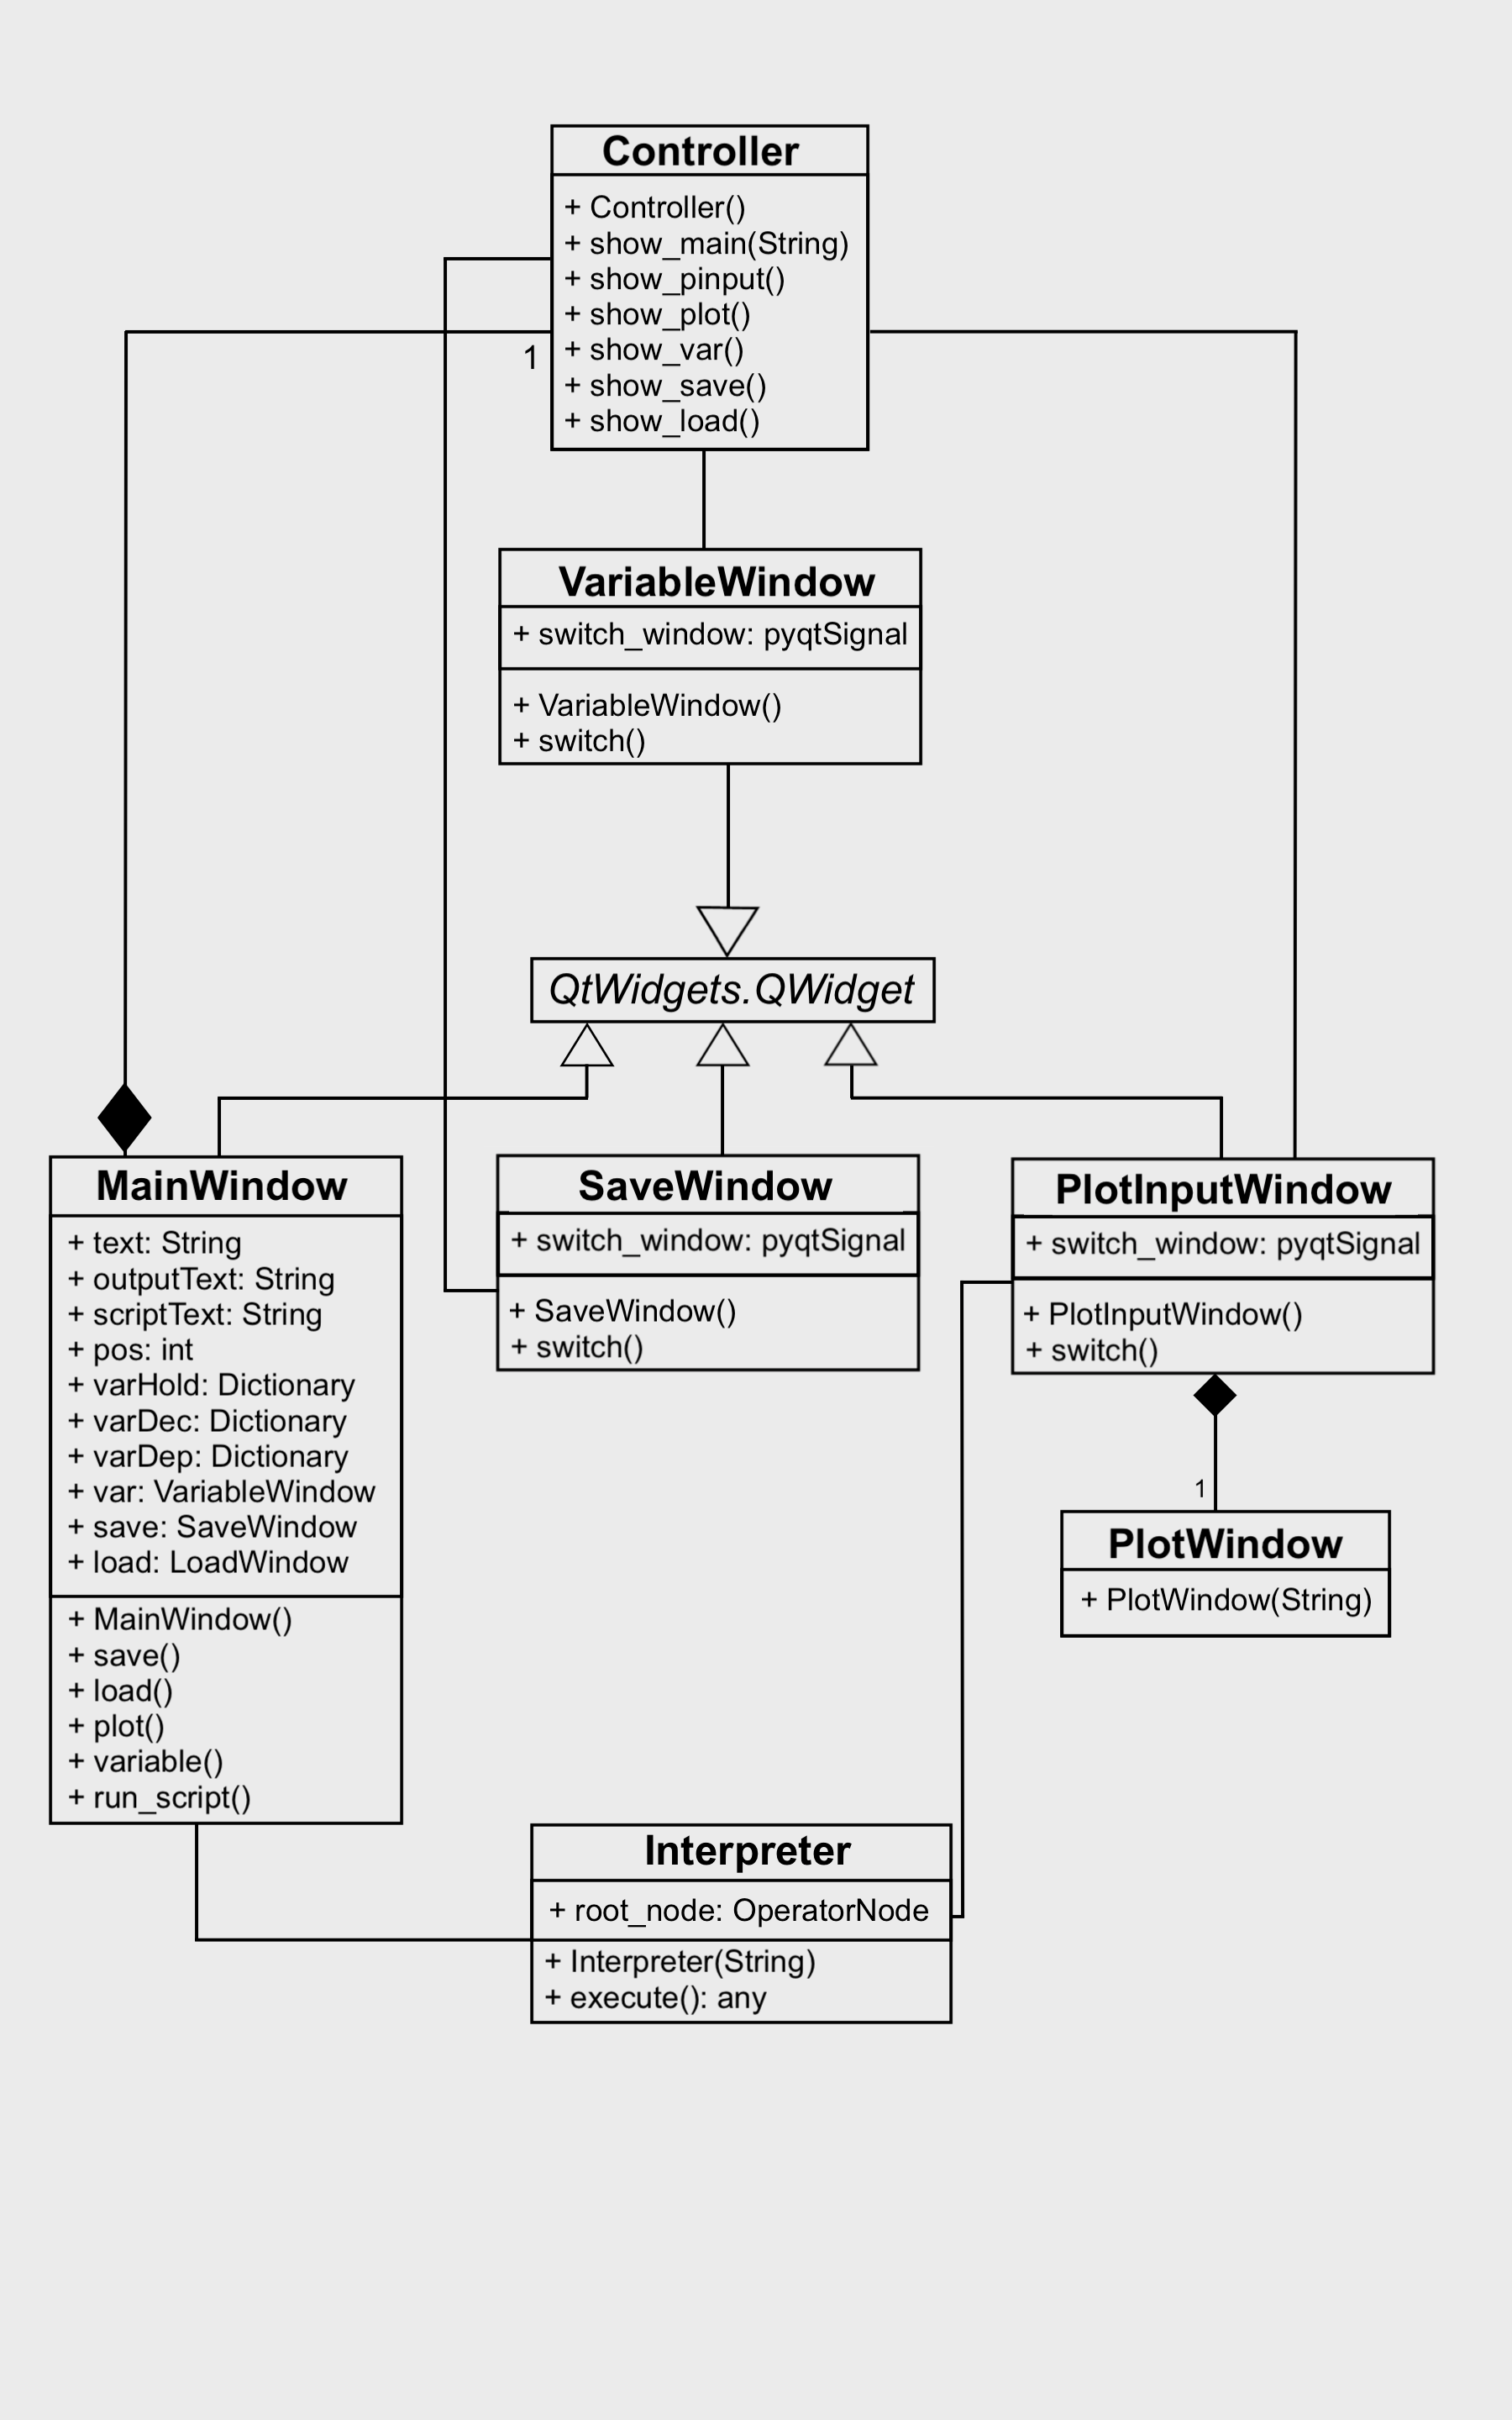
\includegraphics[width=15cm]{UMLClass2.png}
    \caption{UML Class diagram for the GUI}
    \label{fig:UMLClassGUI}
\end{figure}

\newpage

\begin{figure}[H]
    \centering
    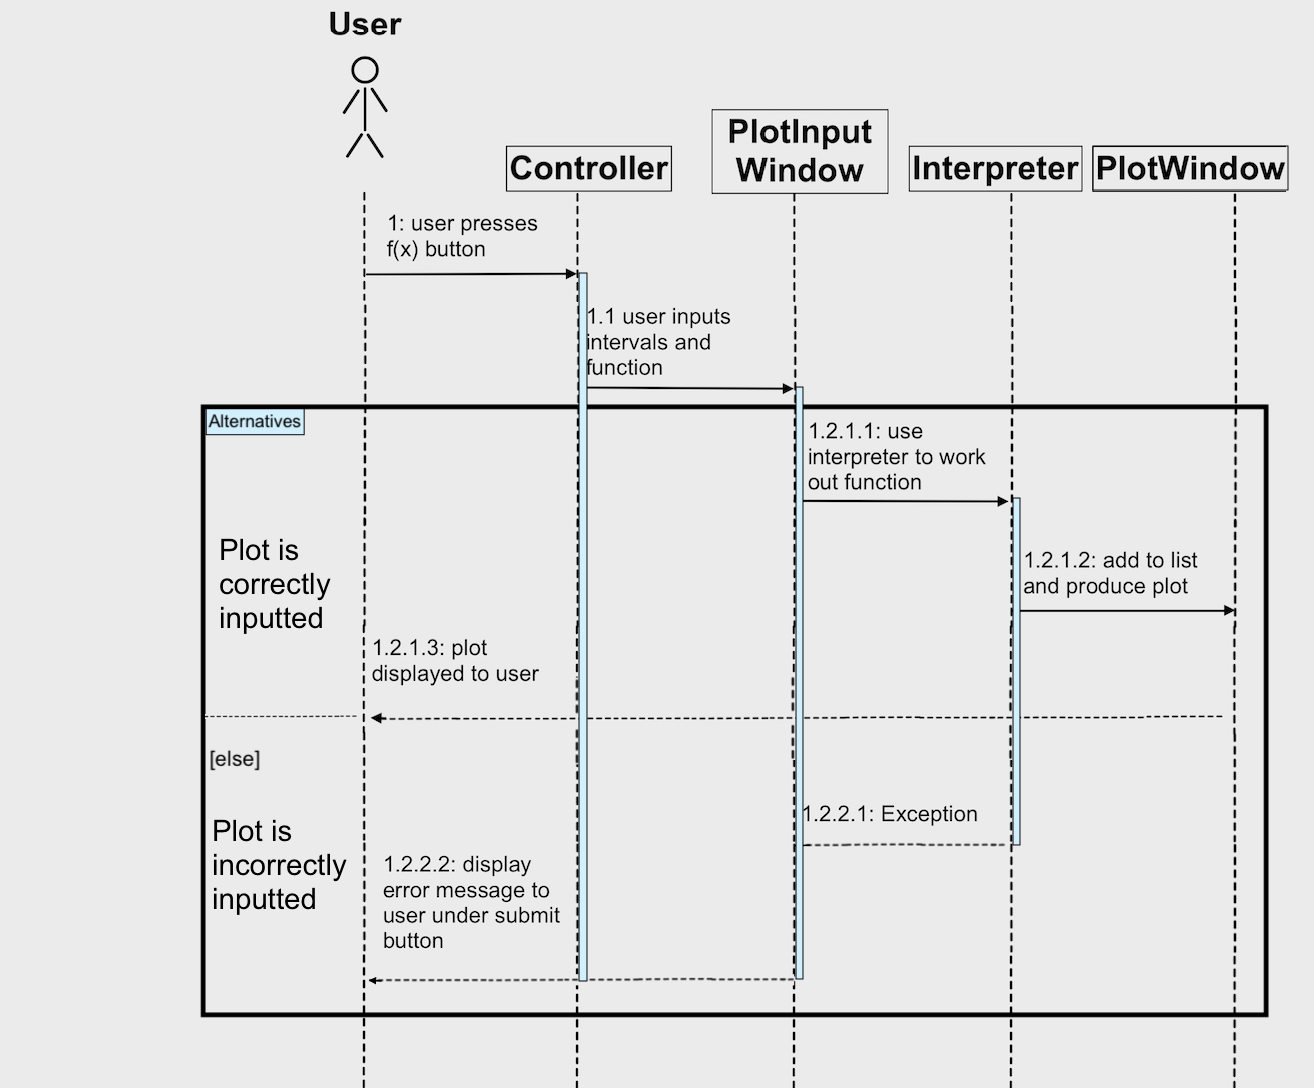
\includegraphics[width=15cm]{UMLSequence.png}
    \caption{UML Class diagram for the GUI}
    \label{fig:UMLSequence}
\end{figure}

\newpage

\section{Gantt Chart}\label{gantt}

\begin{figure}[H]
    \centering
    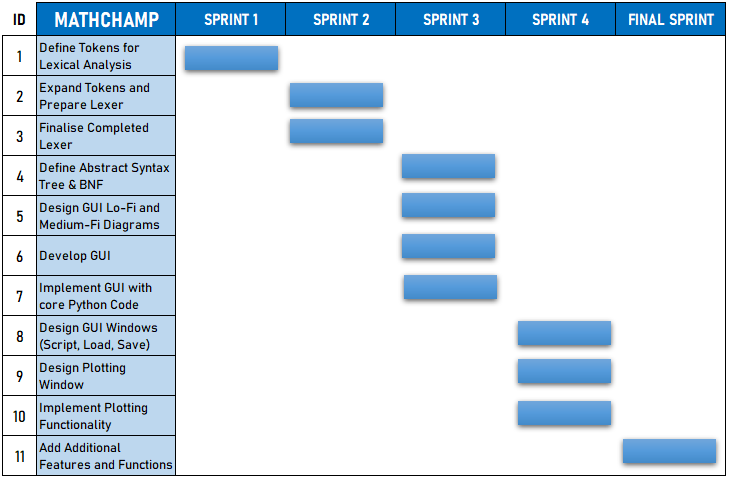
\includegraphics[width=15.5cm]{Gantt.png}
    \caption{MathChamp Development Gantt}
    \label{fig:Gantt}
\end{figure}

\newpage

\section{Manual Test Plans}\label{manual-test}

\begin{figure}[H]
    \centering
    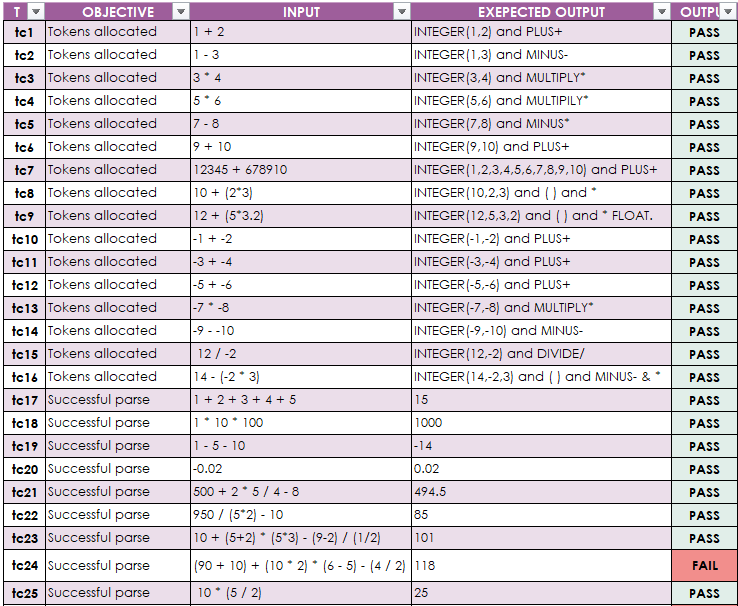
\includegraphics[width=16.0cm]{MathChampTestPlan-A.png}
    \caption{Manual Tests (1 - 25)}
    \label{fig:tests1-25}
\end{figure}
\newpage

\begin{figure}[H]
    \centering
    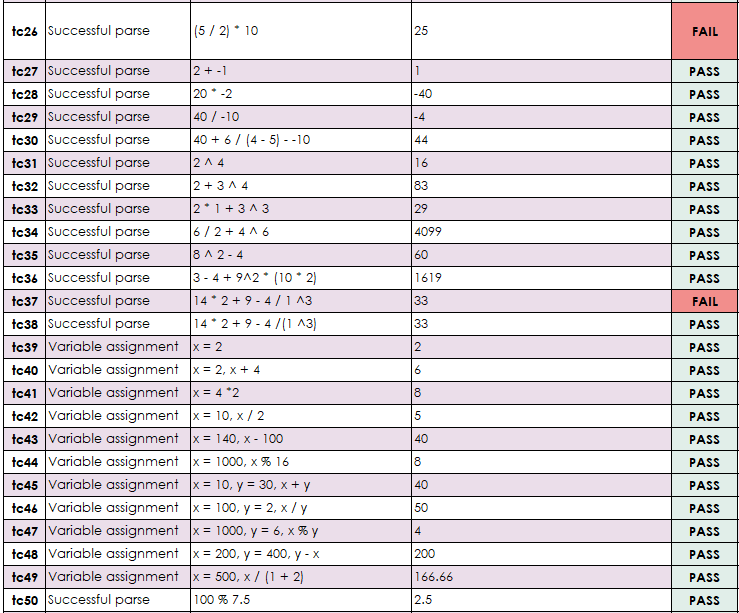
\includegraphics[width=16.0cm]{MathChampTestPlan-B.png}
    \caption{Manual Tests (26 - 50)}
    \label{fig:tests26-50}
\end{figure}
\newpage

\begin{figure}[H]
    \centering
    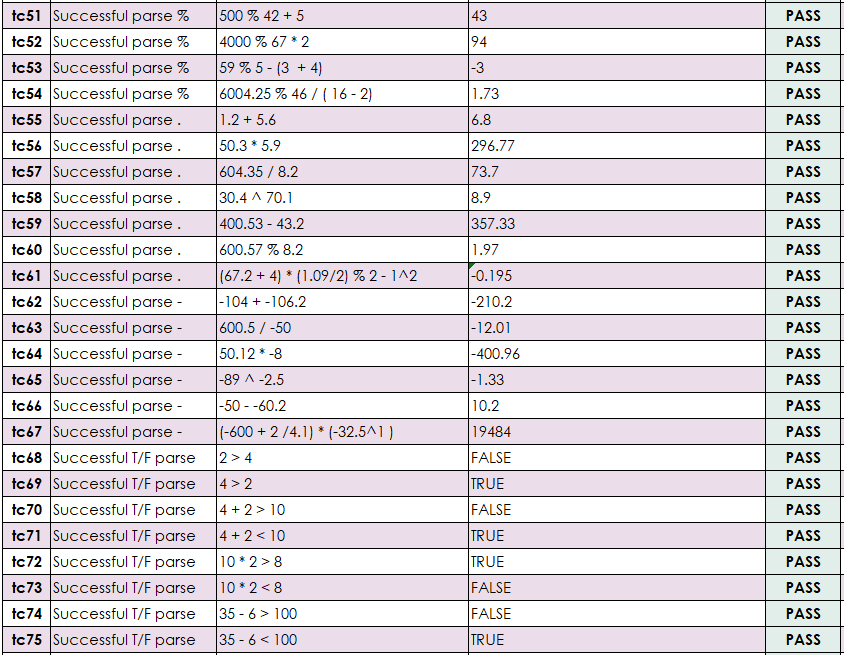
\includegraphics[width=16.0cm]{MathChampTestPlan-C.png}
    \caption{Manual Tests (51 - 75)}
    \label{fig:tests51-75}
\end{figure}
\newpage

\begin{figure}[H]
    \centering
    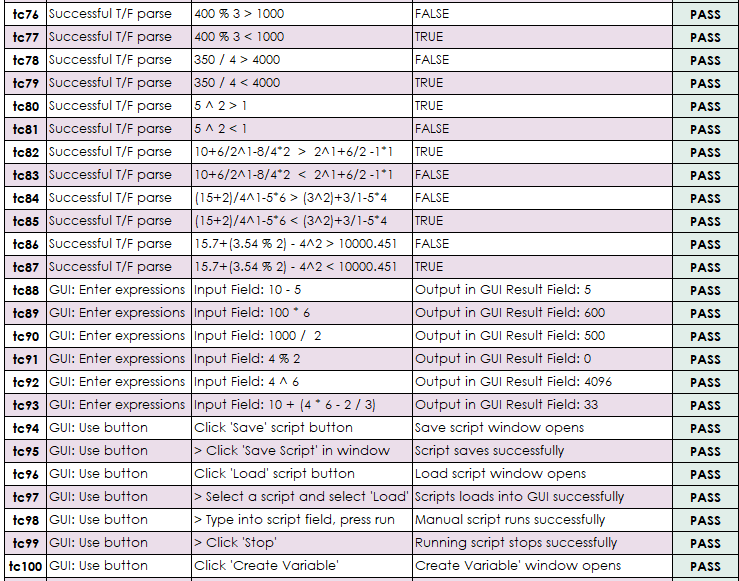
\includegraphics[width=16.0cm]{MathChampTestPlan-D.png}
    \caption{Manual Tests (76 - 100)}
    \label{fig:tests76 - 100}
\end{figure}
\newpage

\begin{figure}[H]
    \centering
    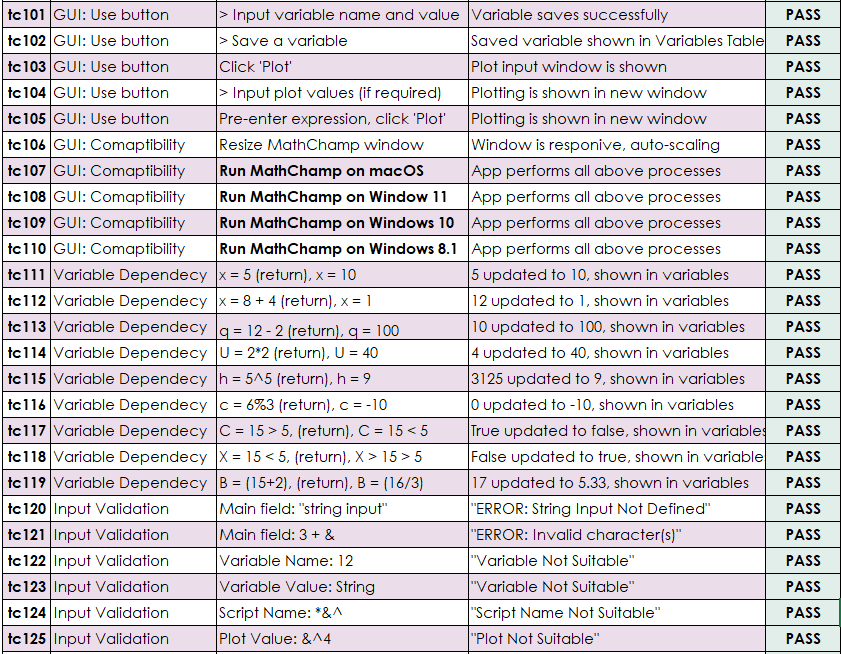
\includegraphics[width=16.0cm]{MathChampTestPlan-E.png}
    \caption{Manual Tests (101 - 125)}
    \label{fig:tests76 - 100}
\end{figure}
\newpage

\end{document}